\documentclass[11pt,oneside,openright]{./style/phdthesis}

\usepackage{amsmath}
\usepackage[ansinew]{inputenc}
\usepackage[portuguese]{babel}
%\usepackage[printonlyused, withpage]{acronym}
\usepackage{a4wide}
\usepackage{palatino}
\usepackage{fancyhdr}
\usepackage{fancybox}
\usepackage{amssymb}
%\usepackage{chapterbib} %com este package as referencias bibliográficas aparecem no final de cada capítulo
\usepackage{cite}
\usepackage{epsfig}
%\usepackage{subfigure}
\usepackage{graphics}
\usepackage{float}
\usepackage{here}
\usepackage[T1]{fontenc}
\usepackage{rotating}
\usepackage{multirow}
%\usepackage{comment}
%\usepackage{captionhack}
\usepackage{epigraph}
\usepackage[linkcolor=black]{hyperref}
%\renewcommand{\thesubfigure}{}
\hypersetup{colorlinks=true}
\usepackage{enumerate}
%\usepackage[numbers,sort&compress]{natbib}
%\usepackage{hypernat}
\usepackage{booktabs}
\usepackage{url}                    % needed to cite a site
\usepackage{eurosym}
\usepackage{makeidx}
\usepackage{datatool}
\usepackage[toc, acronym]{glossaries}
\usepackage{graphicx}
\usepackage{caption}
\usepackage{subcaption}

\usepackage{tabulary}
\usepackage{braket}

% subfile handling packages
\usepackage{subfiles}

\usepackage{multicol} 
\newcommand{\onlyinsubfile}[1]{#1}
\newcommand{\notinsubfile}[1]{}
\renewcommand{\textfraction}{0.01}
\renewcommand{\topfraction}{0.99}
\renewcommand{\floatpagefraction}{0.99}
\renewcommand{\bottomfraction}{0.99}
\renewcommand{\heavyrulewidth}{1pt}
\renewcommand{\lightrulewidth}{0.50pt}
\renewcommand{\chaptername}{Capítulo}
\renewcommand{\figurename}{Figura}
\renewcommand{\appendixname}{\Large{Anexo}}
\renewcommand{\tablename}{Tabela}
\renewcommand{\acronymname}{Acrónimos}

\newcommand{\mli}[1]{\mathit{#1}}
\newcommand{\intSpace}{\!\!\!\!}
\newcommand{\doubleInt}{\!\!\int\intSpace\int\!\!}
\newcommand{\TX}{\mathit{TX}}
\newcommand{\NLI}{\mathit{NLI}}
\newcommand{\eff}{\mathit{eff}}
\newcommand{\LOASE}{\mathit{LO-ASE}}
\newcommand{\LONLI}{\mathit{LO-NLI}}

%\makesavenoteenv{tabular}



\hyphenpenalty=50000
\tolerance=10000
%%% General page formatting

\oddsidemargin 0.2in
\evensidemargin 0in
%\textwidth 155mm
\headheight 15.0pt
\topmargin 0in
%\textheight 237mm

% footheight 1.0in

\makeatletter
\providecommand*{\diff}%
{\@ifnextchar^{\DIfF}{\DIfF^{}}}
\def\DIfF^#1{%
\mathop{\mathrm{\mathstrut d}}%
\nolimits^{#1}\gobblespace}
\def\gobblespace{%
\futurelet\diffarg\opspace}
\def\opspace{%
\let\DiffSpace\!%
\ifx\diffarg(%
\let\DiffSpace\relax
\else
\ifx\diffarg[%
\let\DiffSpace\relax
\else
\ifx\diffarg\{%
\let\DiffSpace\relax
\fi\fi\fi\DiffSpace}

\providecommand*{\tDeriv}[3][]{%
\frac{\diff^{#1}#2}{\diff #3^{#1}}}
\providecommand*{\pDeriv}[3][]{%
\frac{\partial^{#1}#2}%
{\partial #3^{#1}}}

\graphicspath{{./figures/}}


\DeclareMathOperator{\erf}{erf}
\DeclareMathOperator{\erfc}{erfc}
\DeclareMathOperator{\sinc}{sinc}
\DeclareMathOperator{\R}{Re}
\DeclareMathOperator{\I}{Im}
\DeclareMathOperator{\asinh}{asinh}

%\newcommand{\publ}{}

\pagenumbering{arabic}


\makeindex

\begin{document}
%%  include the LaTeX files containing the text for each chapters

% ------------------------------------------------------------------------
\title{NetXPTO - LinkPlanner}
\author{}
\date{\today}
\maketitle
% ------------------------------------------------------------------------

% ------------------------------------------------------------------------
\tableofcontents
% ------------------------------------------------------------------------



% ------------------------------------------------------------------------
\chapter{Introduction}









% ------------------------------------------------------------------------
\chapter{Simulator Structure}

LinkPlanner is a signals open-source simulator.

The major entity is the system.

A system comprises a set of blocks.

The blocks interact with each other through signals.

\section{System}

You can run the System







% ------------------------------------------------------------------------
\chapter{Development Cycle}

The NetXPTO-LinkPlanner has been developed by several people using git as a version control system.
The NetXPTO-LinkPlanner repository is located in the GitHub site http://github.com/netxpto/linkplanner.
The more updated functional version of the software is in the branch master.
Master should be considered a functional beta version of the software.
Periodically new releases are delivered from the master branch under the branch name Release<Year><Month><Day>.
The integration of the work of all people is performed by Armando Nolasco Pinto in the branch Develop.
Each developer has is how branch with his/her name.




\include{chapter/visualizer}

% ------------------------------------------------------------------------
\chapter{Case Studies}

\section{QPSK Transmitter}

This system simulates a QPSK transmitter. A schematic representation of this system is shown in figure \ref{QPSK_transmitter_block_diagram_simple}.

\begin{figure}[h]
	\centering
	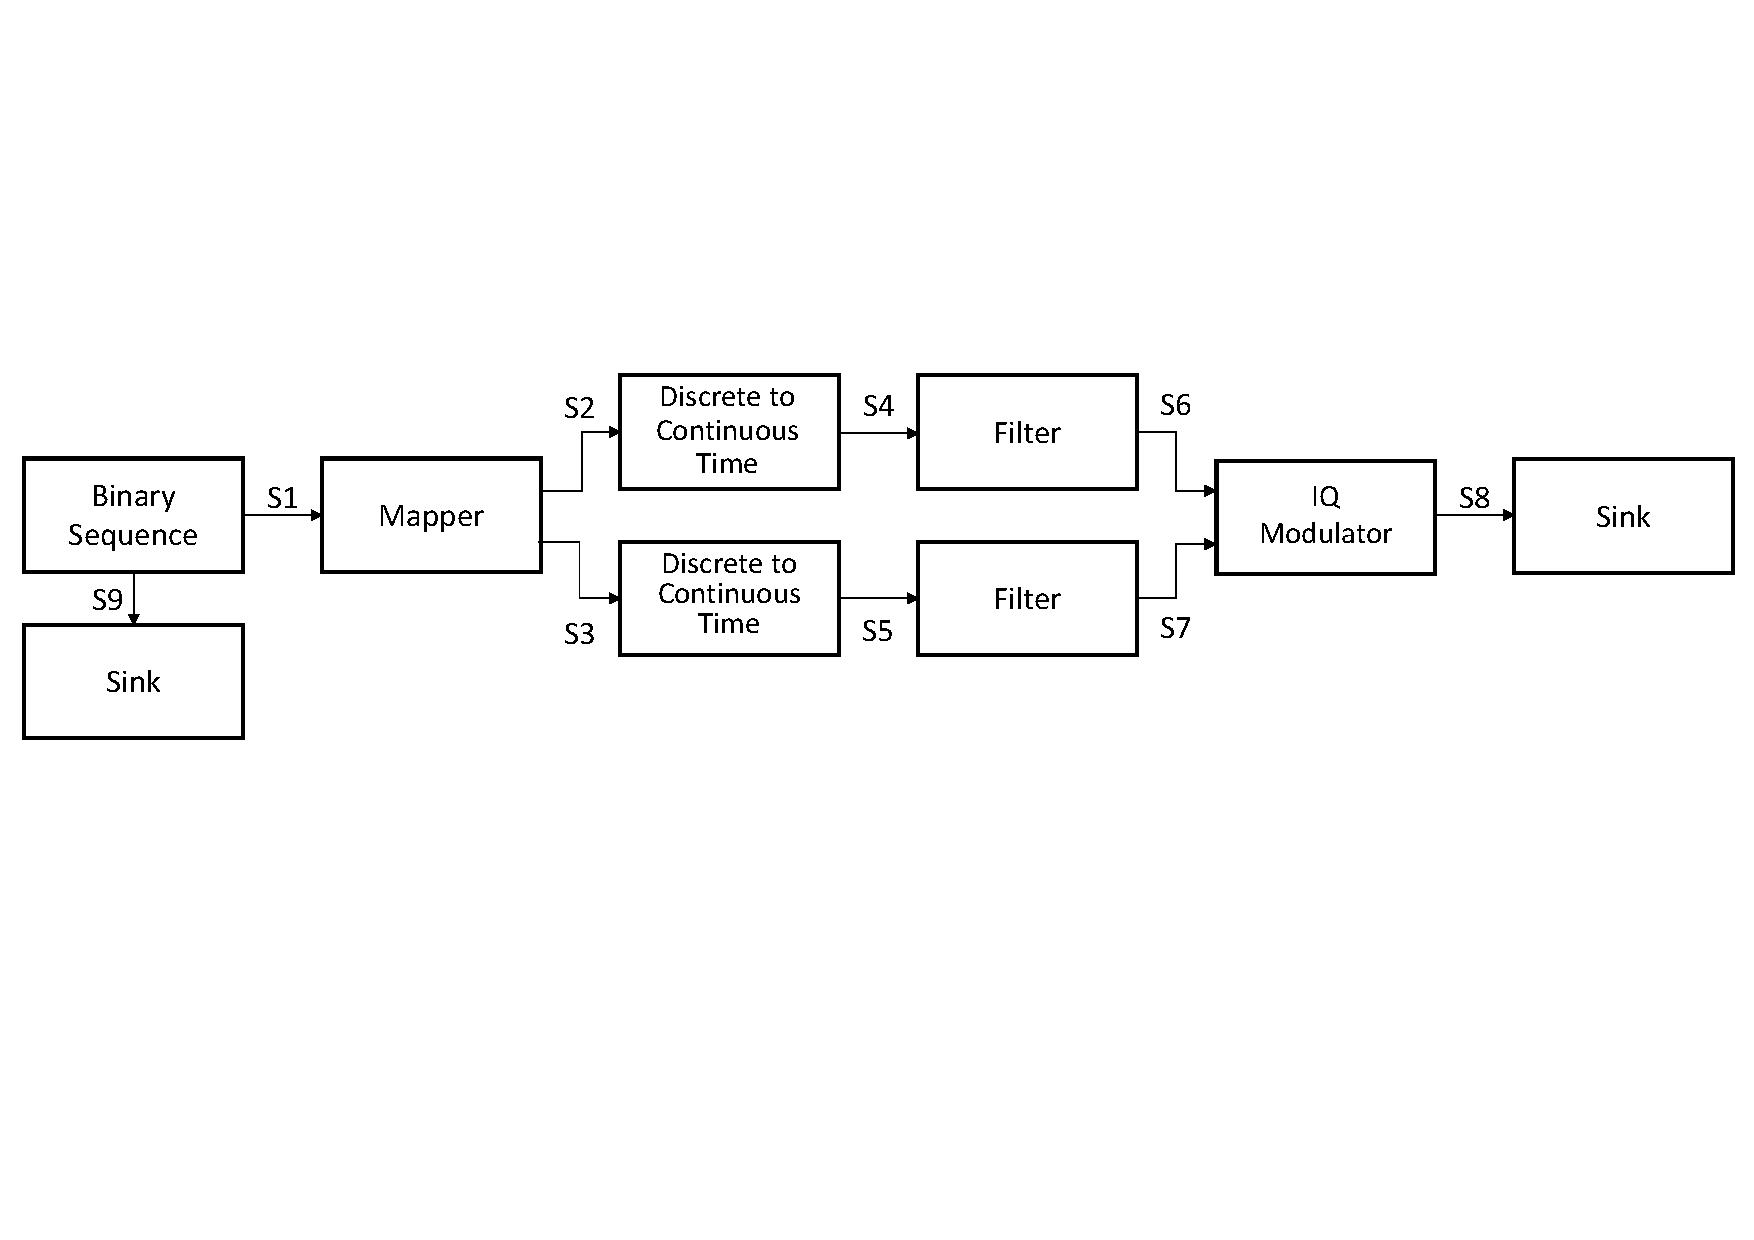
\includegraphics[width=0.5\textwidth]{figures/qpsk_transmitter.pdf}
	\caption{QPSK transmitter block diagram}\label{QPSK_transmitter_block_diagram_simple}
\end{figure}

\subsection*{Functional description}

This block generates an optical signal (output signal 1 in figure \ref{MQAM_transmitter_block_diagram}). The binary signal generated in the internal block Binary Source (block B1 in figure \ref{MQAM_transmitter_block_diagram}) can be used to perform a Bit Error Rate (BER) measurement and in that sense it works as an extra output signal (output signal 2 in figure \ref{MQAM_transmitter_block_diagram}).

\begin{figure}[h]
	\centering
	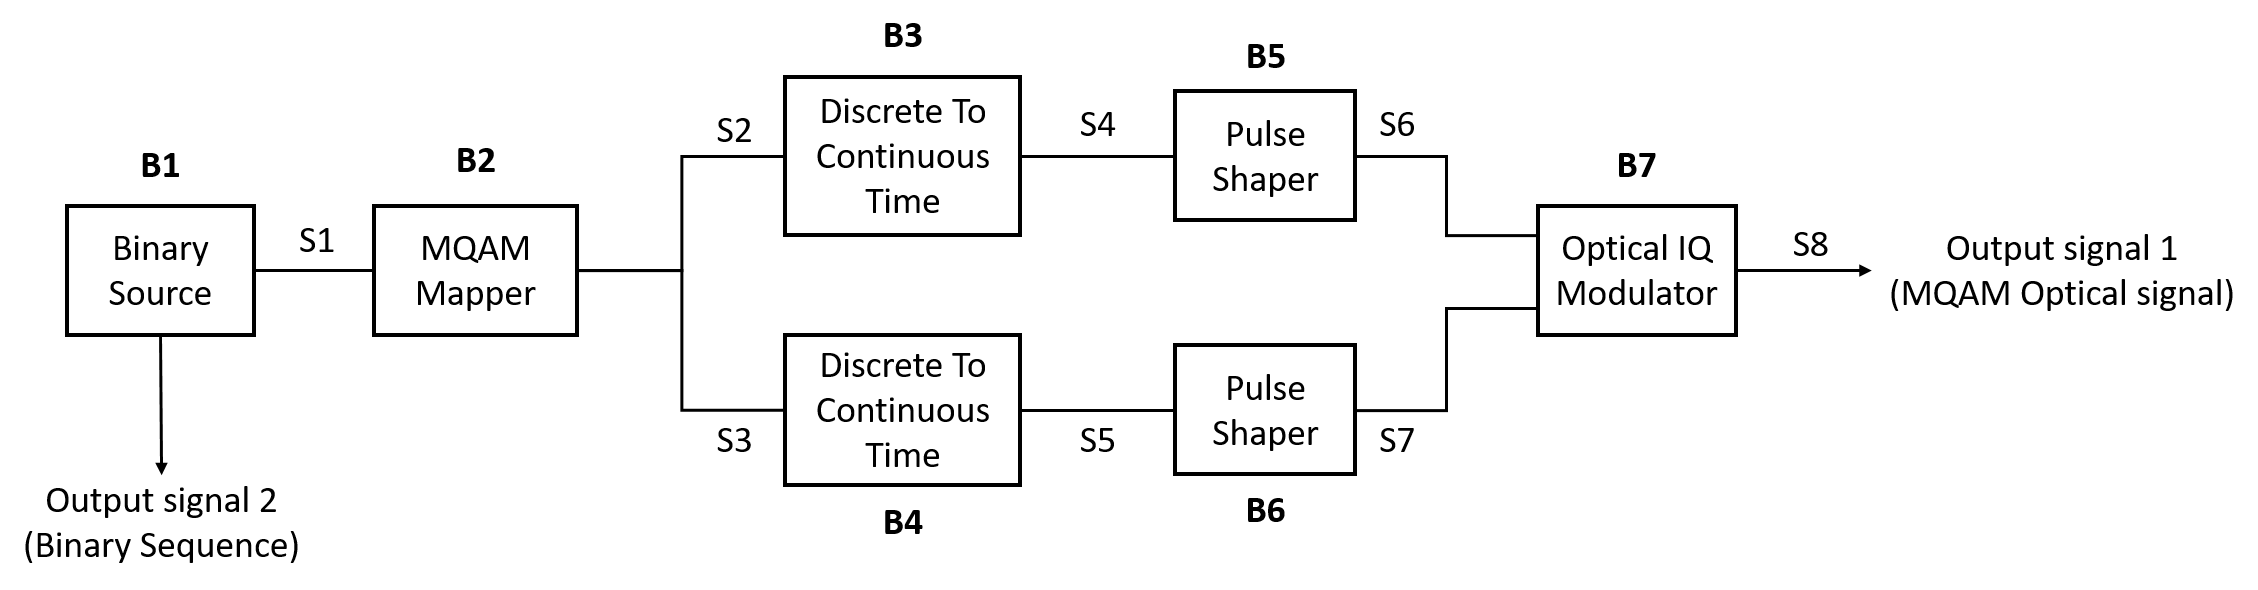
\includegraphics[width=\textwidth]{figures/MQAM_transmitter_block_diagram}
	\caption{Schematic representation of the block MQAM transmitter.}\label{MQAM_transmitter_block_diagram}
\end{figure}

\subsection*{Input parameters}

This block has a special set of functions that allow the user to change the basic configuration of the transmitter. The list of input parameters, functions used to change them and the values that each one can take are summarized in table \ref{table}.

\begin{table}[h]
\begin{center}
	\begin{tabular}{| m{3,5cm} | m{5,1cm} |  m{2,5cm} | m{4cm} | }
		\hline
		\textbf{Input parameters} & \textbf{Function} & Type & \textbf{Accepted values} \\ \hline
		Mode & setMode() & string & PseudoRandom \newline Random \newline DeterministicAppendZeros \newline DeterministicCyclic \\ \hline
		Number of bits generated & setNumberOfBits() & int & Any integer\\ \hline
		Pattern length & setPatternLength() & int & Real number greater than zero\\ \hline
		Number of bits & setNumberOfBits() & long & Integer number greater than zero\\ \hline
		Number of samples per symbol & setNumberOfSamplesPerSymbol() & int & Integer number of the type $2^n$ with n also integer\\ \hline
		Roll of factor & setRollOfFactor() & double & $\in$ [0,1] \\ \hline
		IQ amplitudes & setIqAmplitudes() & Vector of coordinate points in the I-Q plane & \textbf{Example} for a 4-qam mapping: \{ \{ 1.0, 1.0 \}, \{ -1.0, 1.0 \}, \{ -1.0, -1.0 \}, \{ 1.0, -1.0 \} \} \\ \hline
		Output optical power & setOutputOpticalPower() & int & Real number greater than zero\\ \hline
		Save internal signals & setSaveInternalSignals() & bool & True or False\\
		\hline
	\end{tabular}
	\caption{List of input parameters of the block MQAM transmitter} \label{table}
\end{center}
\end{table}

%\begin{itemize}
%	\item setMode(PseudoRandom);
%	\item setBitPeriod(1.0/50e9);
%	\linebreak (double)
%	\item setPatternLength(3);
%	\linebreak (int)
%	\item setNumberOfBits(10000);
%	\linebreak (long)
%	\item setNumberOfSamplesPerSymbol(32);
%	\linebreak (int)
%	\item setRollOffFactor(0.9);
%	\linebreak (double $\in$ [0,1])
%	\item setIqAmplitudes(\{ \{ 1, 1 \}, \{ -1, 1 \}, \{ -1, -1 \}, \{ 1, -1 \} \});
%	\item setOutputOpticalPower\_dBm(0);
%	\item setSaveInternalSignals(true);
%\end{itemize}

\pagebreak

\subsection*{Methods}

MQamTransmitter(vector$<$Signal *$>$ \&inputSignal, vector$<$Signal *$>$ \&outputSignal); (\textbf{constructor})
\bigbreak

void set(int opt);
\bigbreak
void setMode(BinarySourceMode m)
\bigbreak
BinarySourceMode const getMode(void)
\bigbreak
void setProbabilityOfZero(double pZero)
\bigbreak
double const getProbabilityOfZero(void)
\bigbreak
void setBitStream(string bStream)
\bigbreak
string const getBitStream(void)
\bigbreak
void setNumberOfBits(long int nOfBits)
\bigbreak
long int const getNumberOfBits(void)
\bigbreak
void setPatternLength(int pLength)
\bigbreak
int const getPatternLength(void)
\bigbreak
void setBitPeriod(double bPeriod)
\bigbreak
double const getBitPeriod(void)
\bigbreak
void setM(int mValue)
int const getM(void)
\bigbreak
void setIqAmplitudes(vector$<$t\textunderscore iqValues$>$ iqAmplitudesValues)
\bigbreak
vector$<$t\textunderscore iqValues$>$ const getIqAmplitudes(void)
\bigbreak
void setNumberOfSamplesPerSymbol(int n)
\bigbreak
int const getNumberOfSamplesPerSymbol(void)
\bigbreak
void setRollOffFactor(double rOffFactor)
\bigbreak
double const getRollOffFactor(void)
\bigbreak
void setSeeBeginningOfImpulseResponse(bool sBeginningOfImpulseResponse)
\bigbreak
double const getSeeBeginningOfImpulseResponse(void)
\bigbreak
void setOutputOpticalPower(t\textunderscore real outOpticalPower)
\bigbreak
t\textunderscore real const getOutputOpticalPower(void)
\bigbreak
void setOutputOpticalPower\_dBm(t\_real outOpticalPower\_dBm)
\bigbreak
t\_real const getOutputOpticalPower\_dBm(void)
\pagebreak

\subsection*{Output Signals}

\subparagraph*{Number:} 1 optical and 1 binary (optional)

\subparagraph*{Type:} Optical signal

\subsection*{Example}

\begin{figure}[h]
	\centering
	\includegraphics[width=0.8\textwidth]{figures/BinarySource_output}
	\caption{Example of the binary sequence generated by this block for a sequence 0100...}
\end{figure}

\begin{figure}[h]
	\centering
	\includegraphics[width=0.8\textwidth]{figures/IQmodulator0_output}
	\caption{Example of the output optical signal generated by this block for a sequence 0100...}
\end{figure}

\subsection*{Sugestions for future improvement}

Add to the system another block similar to this one in order to generate two optical signals with perpendicular polarizations. This would allow to combine the two optical signals and generate an optical signal with any type of polarization.

\clearpage
\section{Quantum Noise}

\subsection*{Introduction}\label{sec:intro}

This document describes a simple emission and detection system that uses coherent states as it's means?? of transmission???.\\
The transmitted information consists in a binary sequence which is ??translated?? in a sequence of coherent states. In this simulation, the used constellation is formed by the states $\{ \ket{\alpha}, \ket{i\alpha}, \ket{ - \alpha}, \ket{ - i \alpha} \}$, in which $\alpha$ is defined as $\braket{n} = |\alpha|^2$ ($\braket{n}$ is the expected number of photons in a state). (METER MELHOR) \\
\\
One of the main effects studied in this system is quantum noise, which is an intrinsic effect?? to coherent states(VER MARK FOX). In principle???? (VER REFERENCIAS) the variance of a coherent state is given by $\Delta X_1 \Delta X_2 = \frac{1}{4}$.\\
\\
But, given that we combine two photocurrents to obtain an output current, then the total noise will have a combined value of SOMETHING??? Procurar referencias.\\
\\
Therefore, assuming Gaussian?? (WHY GAUSSIAN?) shot noise, for each quadrature we want $\textrm{Var}(X_i) = \frac{1}{4}$ ?????\\
(TENHO DE PROCURAR REFERENCIAS)
\\
\\
In this simulation, we introduce quantum noise in the photodiodes.
We know that a coherent state has an expected number of photons distributed by a Poisson distribution, which has an average number equal to it's variance. Therefore, when the photodiode detects the power of signal, which is proportional to the number of photons, then it's variance must also be proportional to the number of photons.\\
\\
In fact the last step in detecting the resulting signal introduces an difference between currents, but that only will increase the variance. Assuming the independence between detections, and it's intrinsic noise (PROCURAR MELHOR PALEIO), then:
$$
\textrm{Var}(I_{out}) = \textrm{Var}(I_1) + \textrm{Var}(I_2)
$$
Therefore, the best result we can achieve will be $\textrm{Var}(X) = \frac{1}{4}$ ???? (PROCURAR PALEIO SOBRE ISTO)\\
\\
\\
\subsection*{Functional Description}

The simulation setup is described by diagram in figure \ref{fig:setup}. We start by generating a state from one of the four available ones.???? Then, the signal is received in a Hybrid Detector??? where the signal is compared with a local oscillator giving four different signals in it's output. Two of those signals are detected by a photodiode which output will be the difference of the two photocurrents. The other two signals will be also be detected by another photodiode, which will obtain the other quadrature of the signal.????? (TEM QUE FICAR MELHOR EXPLICADO).



\begin{table}[H]
\centering
\begin{tabular}{c|c}
System Blocks          & netxpto Blocks       \\ \hline
- & MQAM \\
- & LocalOscillator \\
- & Hybrid?? \\
- & Photodiode??\\
- & Sampler ??\\
\end{tabular}
\end{table}


\begin{figure}[h]
\centering
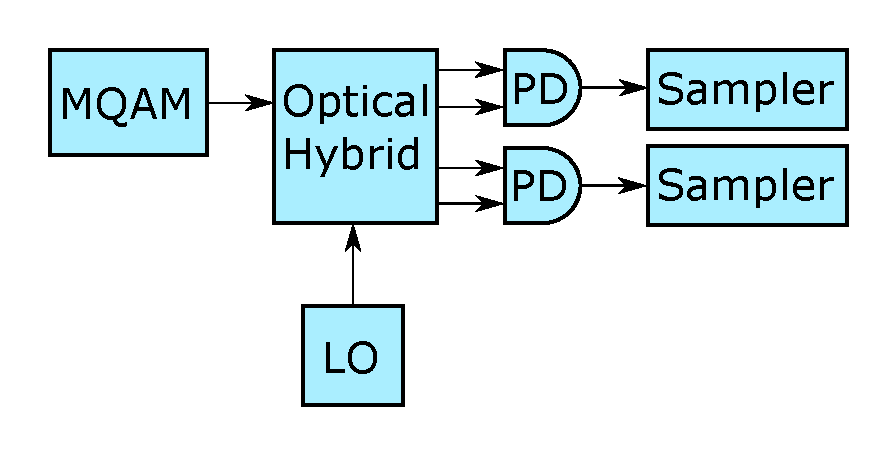
\includegraphics[width=\linewidth]{./sdf/quantum_noise/figures/scheme1.pdf}
\caption{Overview of the optical system being simulated.}
\label{fig:setup}
\end{figure}


\subsection*{Required files}\label{Required files}

Header Files
\begin{table}[H]
\centering
\begin{tabulary}{1.0\textwidth}{|L|L|}
\hline
\textbf{File}           & \textbf{Description}                           \\
\hline
netxpto.h               & Generic purpose simulator definitions.         \\
\hline
m\_qam\_transmitter.h   & ---\\
\hline
local\_oscillator.h     & Generates continuous coherent signal.            \\
\hline
optical\_hybrid.h       & ---\\
\hline
photodiode.h            & ---\\
\hline
sampler.h               & ---\\
\hline
sink.h                  & Closes any unused signals.                       \\
\hline
\end{tabulary}
\end{table}
%
%
Source Files
\begin{table}[H]
\centering
\begin{tabulary}{1.0\textwidth}{|L|L|}
\hline
\textbf{File}                   & \textbf{Description}\\
\hline
netxpto.cpp                     & Generic purpose simulator definitions.\\
\hline
m\_qam\_transmitter.cpp         & ---\\
\hline
local\_oscillator.cpp           & Generates continuous coherent signal.\\
\hline
optical\_hybrid.cpp             & ---\\
\hline
photodiode.cpp                  & ---\\
\hline
sampler.cpp                     & ---\\
\hline
sink.cpp                        & Closes any unused signals.\\
\hline
\end{tabulary}
\end{table}


\subsection*{System Input Parameters}

This system takes into account the following input parameters:
\begin{table}[H]
\centering
\begin{tabulary}{1.0\textwidth}{|C|L|}
\hline
\textbf{System Parameters} & \textbf{Description}\\
\hline
numberOfBitsGenerated   & Gives the number of bits to be simulated\\
\hline
bitPeriod               & Sets the time between adjacent bits\\
\hline
wavelength              & Sets the wavelength of the local oscillator in the MQAM????\\
\hline
samplesPerSymbol        & Establishes the number of samples each bit in the string is given\\
\hline
localOscillatorPower1   & Sets the optical power, in units of W, of the local oscillator inside the MQAM\\
\hline
localOscillatorPower2   & Sets the optical power, in units of W, of the local oscillator used for Bob's measurements\\
\hline
localOscillatorPhase    & Sets the initial phase of the local oscillator used in the detection\\
\hline
transferMatrix          & Sets the transfer matrix of the beam splitter used in the homodyne detector\\
\hline
responsivity            & Sets the responsivity of the photodiodes used in the homodyne detectors\\
\hline
bufferLength            & Sets the length of the buffer used in the signals\\
\hline
iqAmplitudeValues       & Sets the amplitude of the states used in the MQAM????\\
\hline
shotNoise               & Chooses if quantum shot noise is used in the simulation\\
\hline
samplesToSkip			& Sets the number of samples to skip when writing out some of the signal files.\\
\hline
\end{tabulary}
\end{table}		

\subsection*{Inputs}

This system takes no inputs.

\pagebreak
\subsection*{Outputs}

The system outputs the following objects:
\begin{itemize}
\item Signals:
\begin{itemize}
\item Binary Sequence used in the MQAM; (S$_{0}$)
\item Local Oscillator used in the MQAM; (S$_{1}$)
\item Local Oscillator used in the detection; (S$_{2}$)
\item Optical Hybrid Outputs; (S$_{3}$, S$_{4}$, S$_{5}$, S$_{6}$)
\item In phase Photodiode output; (S$_{7}$)
\item Quadrature Photodiode output; (S$_{8}$)
\item In phase Sampler output; (S$_{9}$)
\item Quadrature Sampler output; (S$_{10}$)
\end{itemize}
\end{itemize}	

\subsection*{Simulation Results}\label{subsec:SHresults}

The objective of this simulation was to get the (quantum noise???) associated to the detection of coherent states.\\
\\
\begin{figure}[h]
\centering
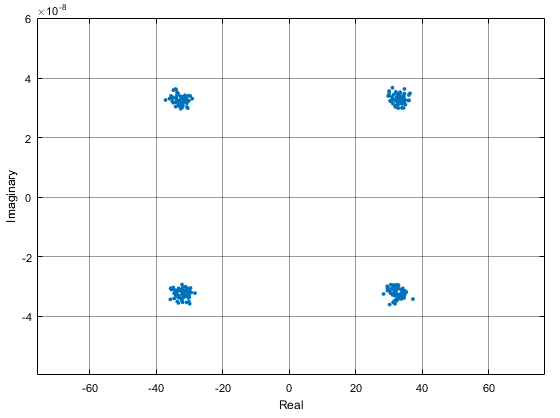
\includegraphics[width=10cm]{./sdf/quantum_noise/figures/constelation1.png}
\caption{Simulation of a constelation of 4 states (n = 100)}
\label{fig:constelation}
\end{figure}
\\
We expect that the variance is invariant with the number of photons sent from Alice. The plot in \ref{fig:variance} show that the simulation also shows this invariance with the number of photons.\\
\begin{figure}[H]
\centering
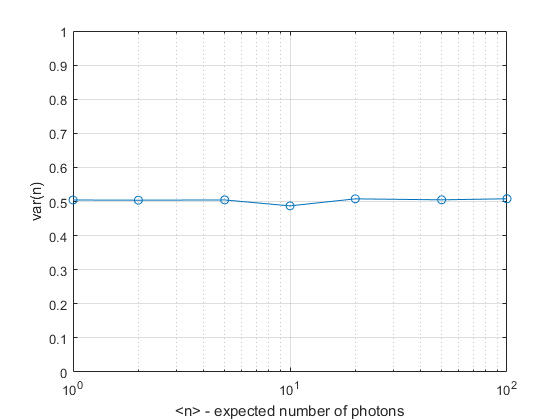
\includegraphics[width=10cm]{./sdf/quantum_noise/figures/variance_n.png}
\caption{Simulation of the variance of $n$.}
\label{fig:variance}
\end{figure}
We can conclude that the expected variance will give us $\textrm{Var(X)} = \frac{1}{2}$.\\
The results obtained in our simulations are in accordance with the theoretical prevision???


%\subsection*{Block Description}
%
%\subsubsection*{MQAM mapper???}
%\subfile{../../lib/tex/m_qam_mapper_v2}
%
%\subsection{Local Oscillator}
%\subfile{../../lib/tex/localoscillator}
%1
%\subsection{Optical Hybrid}
%MISSING FILE FOR OPTICAL HYBRID\\
%%\subfile{../../lib/tex/beamsplitter}
%
%\subsection{Photodiode}
%\subfile{../../lib/tex/photodiode}
%
%\subsection{Sampler}
%\subfile{../../lib/tex/sampler}

\subsection*{Known Problems}
\begin{enumerate}
    \item ----
\end{enumerate}


%\documentclass[a4paper]{article}
%
%% subfile handling packages
%\usepackage{subfiles}
%\newcommand{\onlyinsubfile}[1]{#1}
%\newcommand{\notinsubfile}[1]{}
%
%% document packages
%\usepackage[top=1in, bottom=1.25in, left=1.25in, right=1.25in]{geometry}
%\usepackage{amsmath}
%\usepackage{multicol}
%\usepackage{caption}
%\usepackage{subcaption}
%\usepackage{graphicx}
%\usepackage{multirow}
%\usepackage{tabulary}
%\usepackage{hhline}
%\usepackage{indentfirst}
%\RequirePackage{ltxcmds}[2010/12/07]
%\graphicspath{{../../images/}}
%%\graphicspath
%\usepackage{float}
%\usepackage{amsfonts}
%\usepackage{hyperref}
%\usepackage{footnote}
%\makesavenoteenv{tabular}
%\usepackage{braket}
%%opening
%\title{Safety study}
%\author{}
%\date{}
%
%
%\begin{document}
%\maketitle
\clearpage
\section{Continuos Variable Quantum Transmission System}\label{sec:intro}

In this section a continuous varible quantum transmission system is analyzed.
The results here presented follow closely the~\cite{namiki2003security}.
In~\cite{namiki2003security}, the security of a continuous variable quantum key distribution (CV-QKD) system is studied theoretically, here we complete that theoretical study with simulations results.

\begin{figure}[h]
\centering
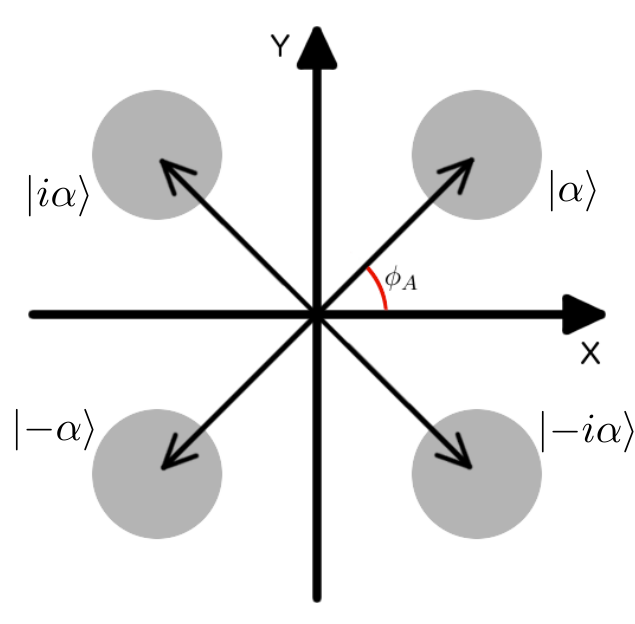
\includegraphics[width=.5\linewidth]{./sdf/cv_system/figures/constellation.png}
\caption{State constellation}
\label{fig:const}
\end{figure}

The state constellation used in the system is presented in Figure~\ref{fig:const}.
The emitter (usually named Alice) is going to use two basis, the $45º$ base and the $-45º$ base.
In the $45º$ base, Alice sends one of two values, $1$ and $-1$, which correspond to the states $\ket{\alpha}$ and $\ket{-\alpha}$.
In the $-45º$ base, Alice can also send one of two values, $1$ and $-1$, which correspond to the states $\ket{-i\alpha}$ and $\ket{i\alpha}$.
At the end Alice is going to send one of the four states $\ket{\alpha}$, $\ket{-\alpha}$, $\ket{-i\alpha}$, and $\ket{i\alpha}$, with equal probability.

Because we don't know $\grave{a}$ prior which state is going be transmitted, neither which basis is going to be used, and to incorporate our ``ignorance"\, in the system description, we can work with the density operator. The density operator is a proper tool to describe ``statistical mixtures". A ``statistical mixtures" is one state, from a possible set, but we don't know which state it is. There is no state superposition.

Since all states have the same probability of occurring, the state density operator is given by:

\begin{equation}\label{eq:statedensity}
\hat{\rho}=\frac{1}{4}\left(\ket{\alpha}\bra{\alpha}+\ket{-\alpha}\bra{-\alpha}+\ket{i\alpha}\bra{i\alpha}+\ket{-i\alpha}\bra{-i\alpha}\right).
\end{equation}

The probability to detect at the receiver the state $\ket{\alpha}$ is given by
\begin{equation}\label{eq:statedensity}
P(\alpha)=\bra{\alpha}\hat{\rho}\ket{\alpha}=\frac{1}{4}.
\end{equation}


Note that the density operator is equivalent to the wave function in terms of the system description.

From the receiver perspective, i.e. from the Bob perspective, and after knowing the base used by Alice.
The density operator can be reduce to,

\begin{align}
\hat{\rho}_1&=\frac{1}{2}\left(\ket{\alpha}\bra{\alpha}+\ket{-\alpha}\bra{-\alpha}\right),\label{eq:statedensity1} \\
\hat{\rho}_2&=\frac{1}{2}\left(\ket{i\alpha}\bra{i\alpha}+\ket{-i\alpha}\bra{-i\alpha}\right).\label{eq:statedensity2}
\end{align}

where $1$ corresponds to the $45º$ base and $-1$ corresponds to $-45º$.

\subsubsection*{Single Base Homodyne Detection}


The probability of obtaining a quadrature $\hat{X}_\phi=\hat{X}_1\cos\phi+\hat{X}_2\sin\phi$ when measuring the coherent state $\ket{\alpha}$ is given by the following gaussian distribution:

\begin{equation}
\left|\braket{X_\phi|\alpha}\right|^2=\sqrt{\frac{2}{\pi}}e^{-2(X_\phi-\alpha\cos\phi)^2},
\end{equation}

We can define the "correct" and "wrong" basis measurement probability density, respectively, as:

\begin{equation}\label{eq:probdensity}
\bra{X_i}\hat{\rho}_j\ket{X_i}=
\begin{cases}
\frac{1}{\sqrt{2\pi}}\left(e^{-2(X_i-\alpha)^2}+e^{-2(X_i+\alpha)}\right), & i=j\\
\sqrt{\frac{2}{\pi}}e^{-2X_i^2}, &i\neq j
\end{cases}.
\end{equation}

The post selection efficiency (PSE) can be defined as the probability of a measurement in the correct basis yields a result that satisfies the limit value $X_0$:

\begin{equation}\label{eq:postselecteff}
\begin{aligned}
P(X_0,\alpha)&=\int^{-X_0}_{-\infty}\bra{X_1}\hat{\rho}_1\ket{X_1}dX_1+\int^{\infty}_{X_0}\bra{X_1}\hat{\rho}_1\ket{X_1}dX_1\\
&=\frac{1}{2}\left[\text{erfc}(\sqrt{2}(X_0+\alpha))+\text{erfc}(\sqrt{2}(X_0-\alpha))\right].
\end{aligned}
\end{equation}

The bit error rate (BER) is the normalized probability of, after choosing the correct basis, obtaining the wrong bit value:

\begin{equation}\label{eq:biterrorratio}
Q(X_0,\alpha)=\frac{1}{P(X_0,\alpha)}\int_{-\infty}^{-X_0}\left|\braket{X_i|\alpha}\right|dX_i=\frac{\text{erfc}\left(\sqrt{2}(X_0+\alpha)\right)}{2P(X_0,n)}
\end{equation}

\begin{figure}[h]
\centering
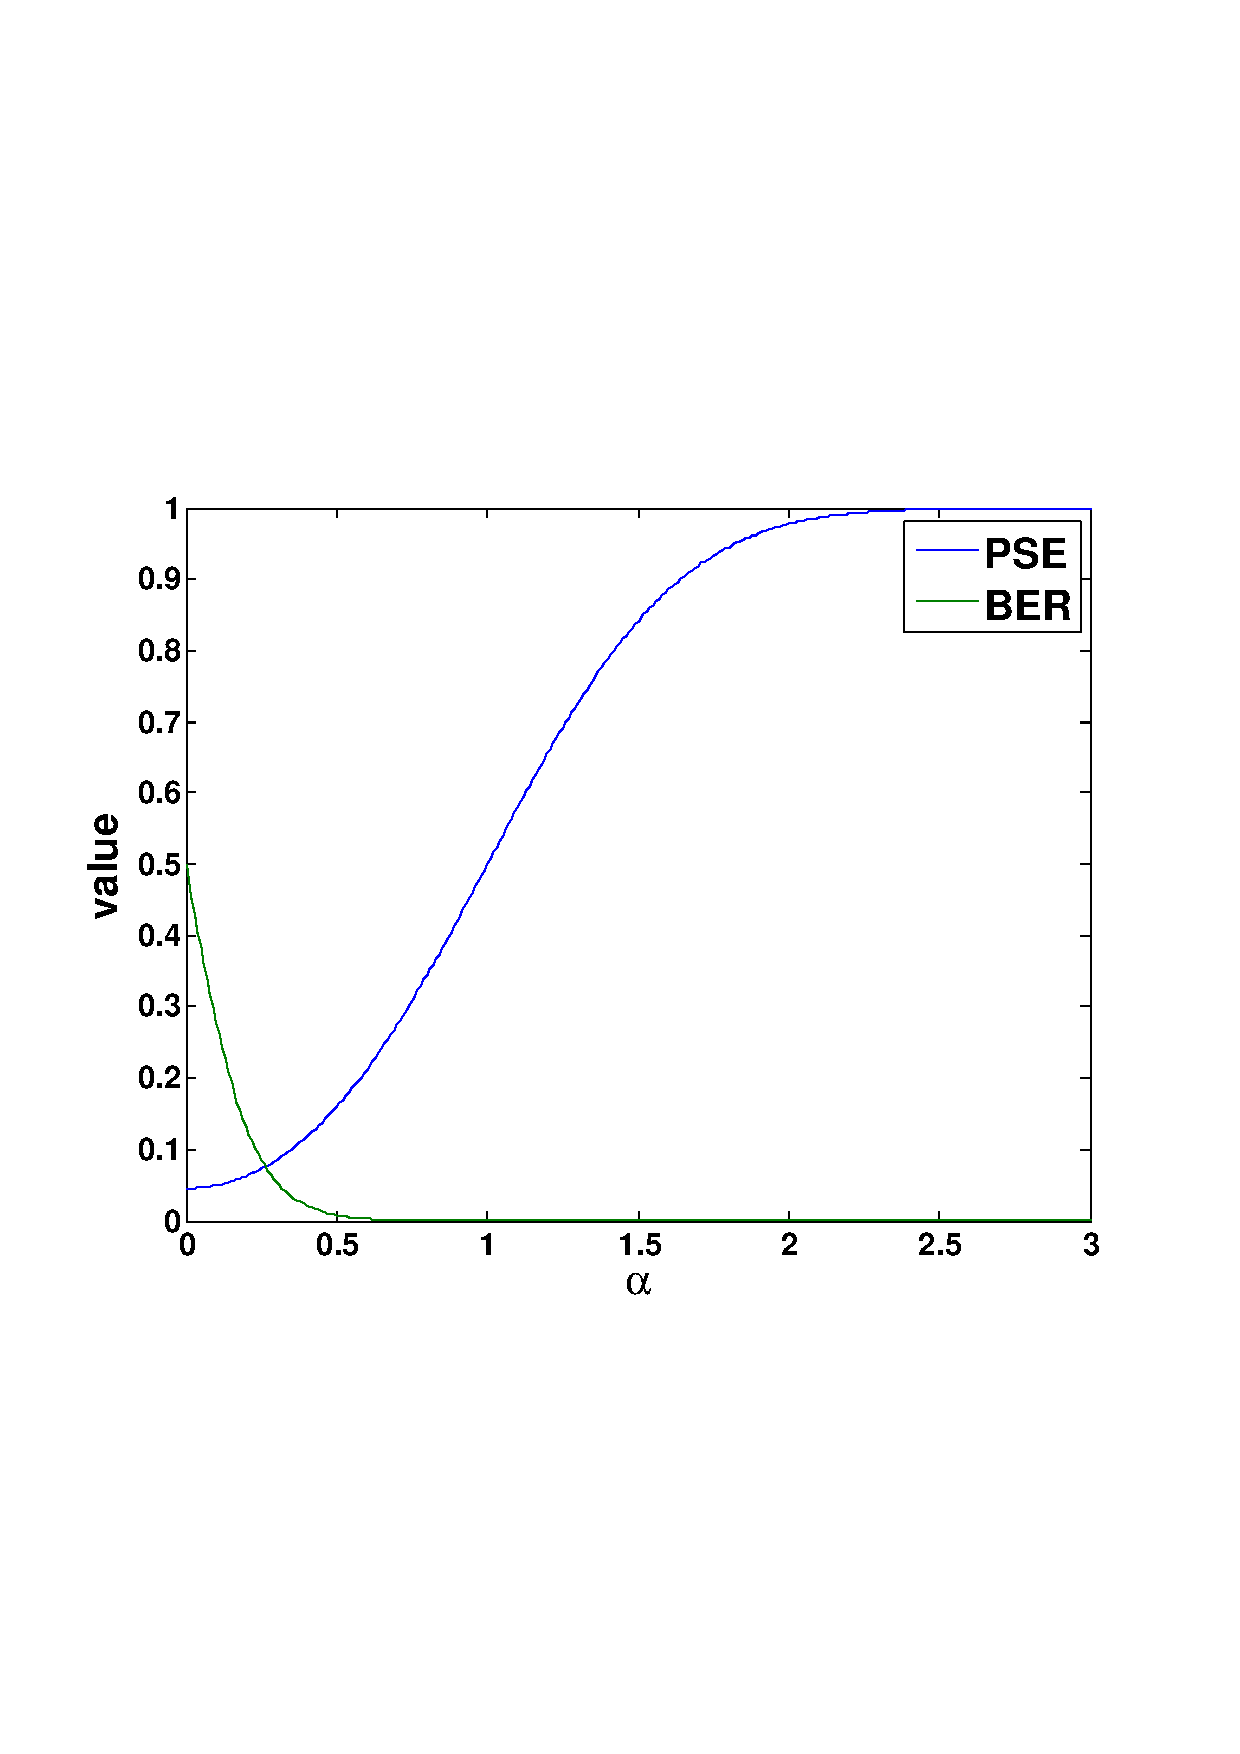
\includegraphics[width=\linewidth, trim= 0mm 60mm 0mm 70mm]{./sdf/cv_system/figures/singlehomodyne.pdf}
\caption{BER and PSE in function of $\alpha$ for the single homodyne setup. $X_0=1$ was used}
\label{fig:ber}
\end{figure}



\subsubsection*{Double Homodyne setup}

In our proposed double homodyne protocol both quadratures are measured simultaneously, as such the concept of correct and wrong basis measurements has no value. Our protocol also makes use of a locally generated Local Oscillator (LO), obtained from a different laser than the one used to generate the signal, thus we have to take into account the phase drift between both lasers. High intensity reference pulses are sent periodically to allow for an estimation of the phase drift. The double homodyne setup requires the signal to be divided into the two utilized detectors, so each measurement is made on a coherent state with half the amplitude of the incoming signal $\alpha\rightarrow\frac{\alpha}{\sqrt{2}}$
\par
For each incoming pulse we measure quadratures $X_\phi$ and $Y_\phi$. $\phi$ has contributions from both the encoded angle, $\theta$, and the phase difference between lasers, $\epsilon$, we assume $\phi=\theta+\epsilon$. On the reference pulses no phase is encoded, that is $\theta=0$, thus $\epsilon$ can be estimated. Assuming $\epsilon$ doesn't change between a reference pulse and the following signal pulse, the measured quadratures can be cast into the originally sent quadratures $X_\theta$ and $Y_\theta$ via:
\begin{equation}
\begin{aligned}
X_\theta&=X_\phi\cos\epsilon-Y_\phi\sin\epsilon\\
Y_\theta&=X_\phi\sin\epsilon+Y_\phi\sin\epsilon
\end{aligned}
\end{equation}
Assuming an announcement of the coding basis, the density operators~\eqref{eq:statedensity1} and~\eqref{eq:statedensity2} still apply. We can now define the probability density of obtaining results $X_\theta$ and $Y_\theta$, assuming a state in the $X_1$ base was sent, as:
\begin{align}
\braket{X_\theta|\hat{\rho}_1|X_\theta}&= \frac{\sqrt{\frac{2}{\pi}}}{4}\left(e^{-2\left(x_\theta-\frac{\alpha}{\sqrt{2}}\cos\theta\right)^2}+e^{-2\left(x_\theta+\frac{\alpha}{\sqrt{2}}\cos\theta\right)^2}\right),\\
\braket{Y_\theta|\hat{\rho_1}|Y_\theta}&= \frac{\sqrt{\frac{2}{\pi}}}{4}\left(e^{-2\left(y_\theta-\frac{\alpha}{\sqrt{2}}\sin\theta\right)^2}+e^{-2\left(y_\theta+\frac{\alpha}{\sqrt{2}}\sin\theta\right)^2}\right).
\end{align}
\par
Now each state needs to satisfy two limit values, $X_0$ and $Y_0$, to be accepted. Thus, the PSE is now defined as:
\begin{equation}
\begin{aligned}
P_{DH}(X_0,Y_0,\alpha)&=\int^{-X_0}_{-\infty}\braket{X_\theta|\hat{\rho}_1|X_\theta}dx_\theta\int^{-Y_0}_{-\infty}\braket{Y_\theta|\hat{\rho}_1|Y_\theta}dy_\theta+\\
&\int_{X_0}^{\infty}\braket{X_\theta|\hat{\rho}_1|X_\theta}dx_\theta\int_{Y_0}^{\infty}\braket{Y_\theta|\hat{\rho}_1|Y_\theta}dy_\theta\\
&=\frac{1}{4}\left\lbrace\text{erfc}\left[\sqrt{2}\left(X_0-\frac{\alpha}{\sqrt{2}}\cos\theta\right)\right]+\text{erfc}\left[\sqrt{2}\left(X_0+\frac{\alpha}{\sqrt{2}}\cos\theta\right)\right]\right\rbrace\\
&\left\lbrace\text{erfc}\left[\sqrt{2}\left(Y_0-\frac{\alpha}{\sqrt{2}}\sin\theta\right)\right]+\text{erfc}\left[\sqrt{2}\left(Y_0+\frac{\alpha}{\sqrt{2}}\sin\theta\right)\right]\right\rbrace,
\end{aligned}
\end{equation}
The DH subscript denotes Double Homodyne. In a somewhat similar manner, the BER is now defined as:
\begin{equation}\label{eq:adaptedBER}
\begin{aligned}
Q_{DH}(X_0,Y_0,\alpha)&=\frac{1}{P_{DH}}\left(\int^{-X_0}_{-\infty}\left|\braket{X_\theta|\frac{\alpha}{\sqrt{2}}}\right|^2dx_\theta\int^{-Y_0}_{-\infty}\left|\braket{Y_\theta|\frac{\alpha}{\sqrt{2}}}\right|^2dy_\theta+\right.\\
&\left.\int_{X_0}^{\infty}\left|\braket{X_\theta|-\frac{\alpha}{\sqrt{2}}}\right|^2dx_\theta\int_{Y_0}^{\infty}\left|\braket{Y_\theta|-\frac{\alpha}{\sqrt{2}}}\right|^2dy_\theta\right)\\
&=\frac{1}{2P_{DH}}\text{erfc}\left[\sqrt{2}\left(X_0+\frac{\alpha}{\sqrt{2}}\cos\theta\right)\right]\text{erfc}\left[\sqrt{2}\left(Y_0+\frac{\alpha}{\sqrt{2}}sin\theta\right)\right],
\end{aligned}
\end{equation}
note that, in this definition for BER, only values $\theta\in\left[0,\frac{\pi}{2}\right]$ make sense (the sent state was $\alpha$).

\begin{figure}[h]
\centering
\begin{subfigure}{.48\linewidth}
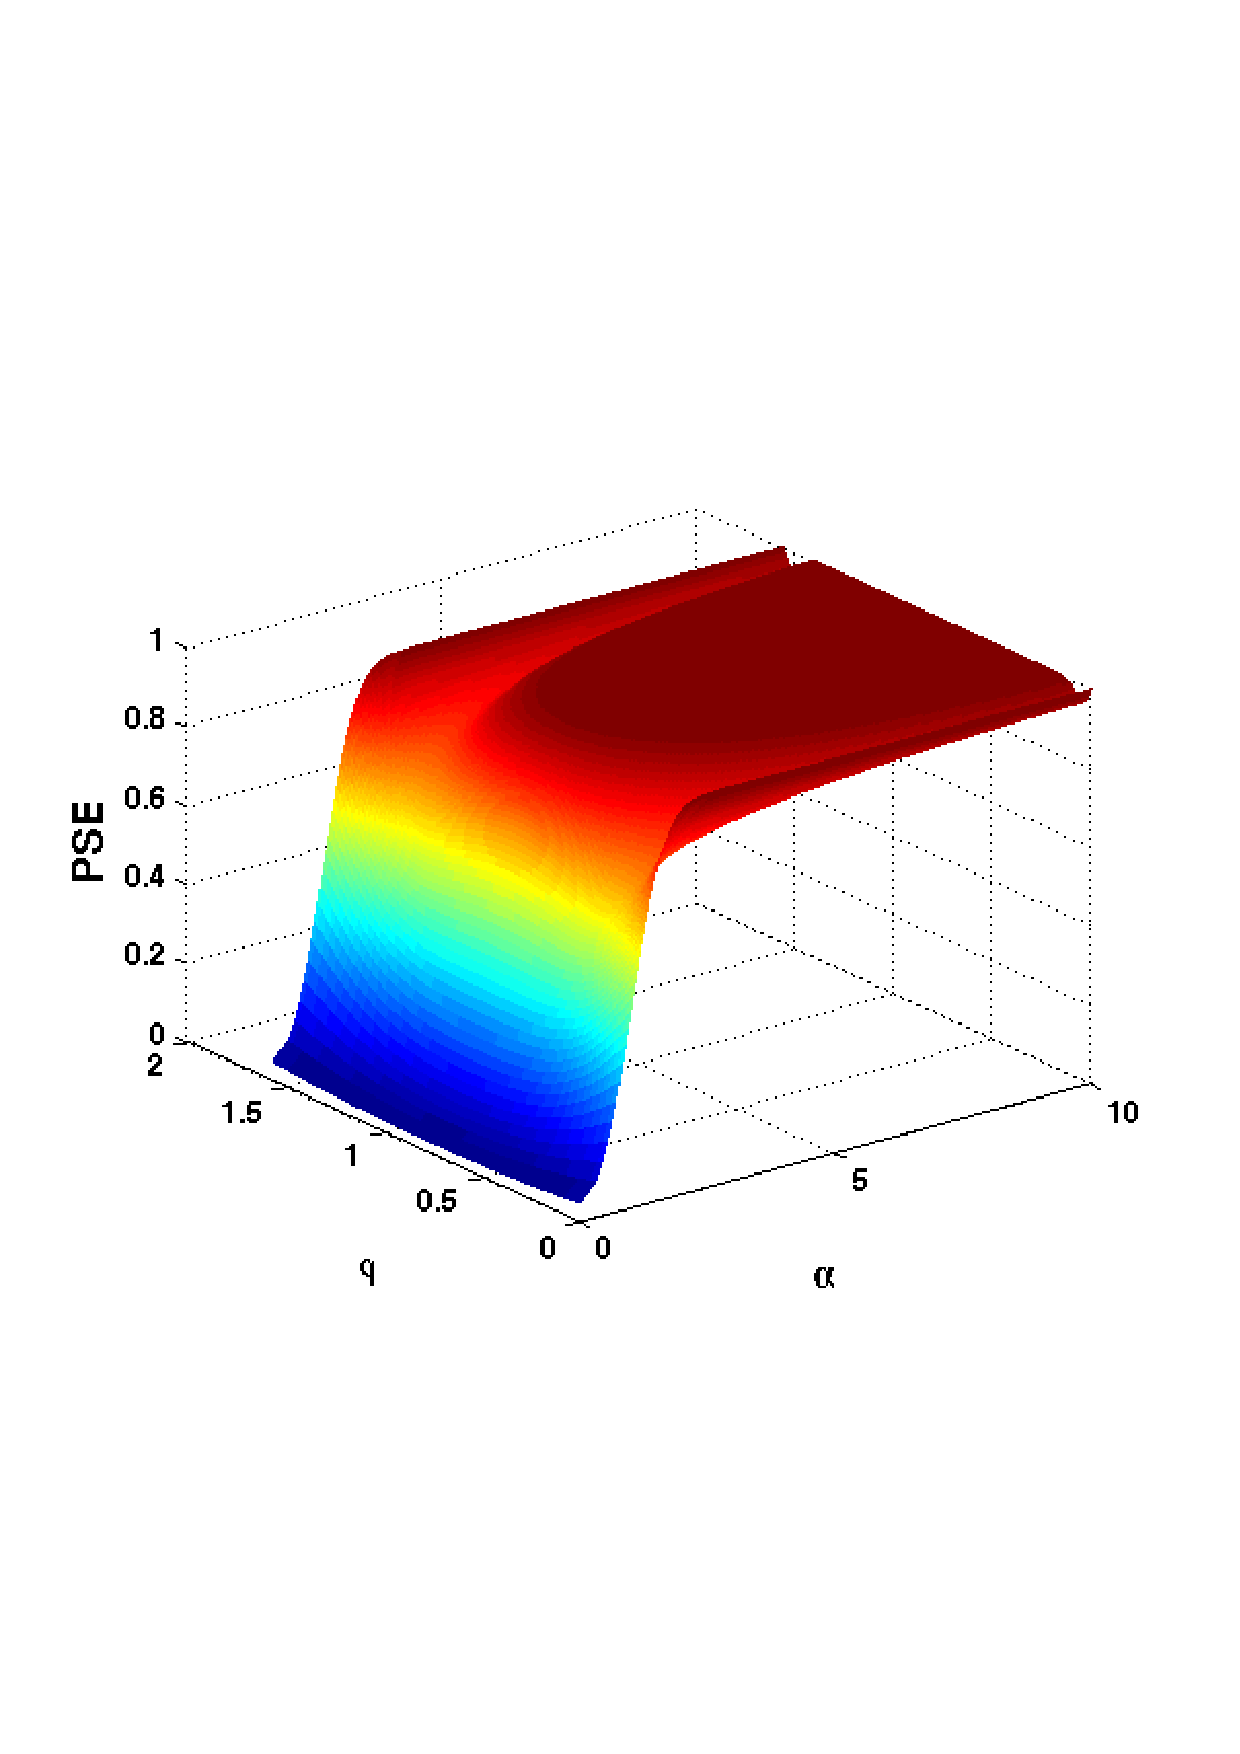
\includegraphics[width=\linewidth, trim= 0mm 60mm 0mm 70mm]{doublehomodynePSE.pdf}
\caption{PSE in function of $\alpha$ and $\theta$ for the double homodyne setup. $X_0=1$ was used}
\end{subfigure}
~
\begin{subfigure}{.48\linewidth}
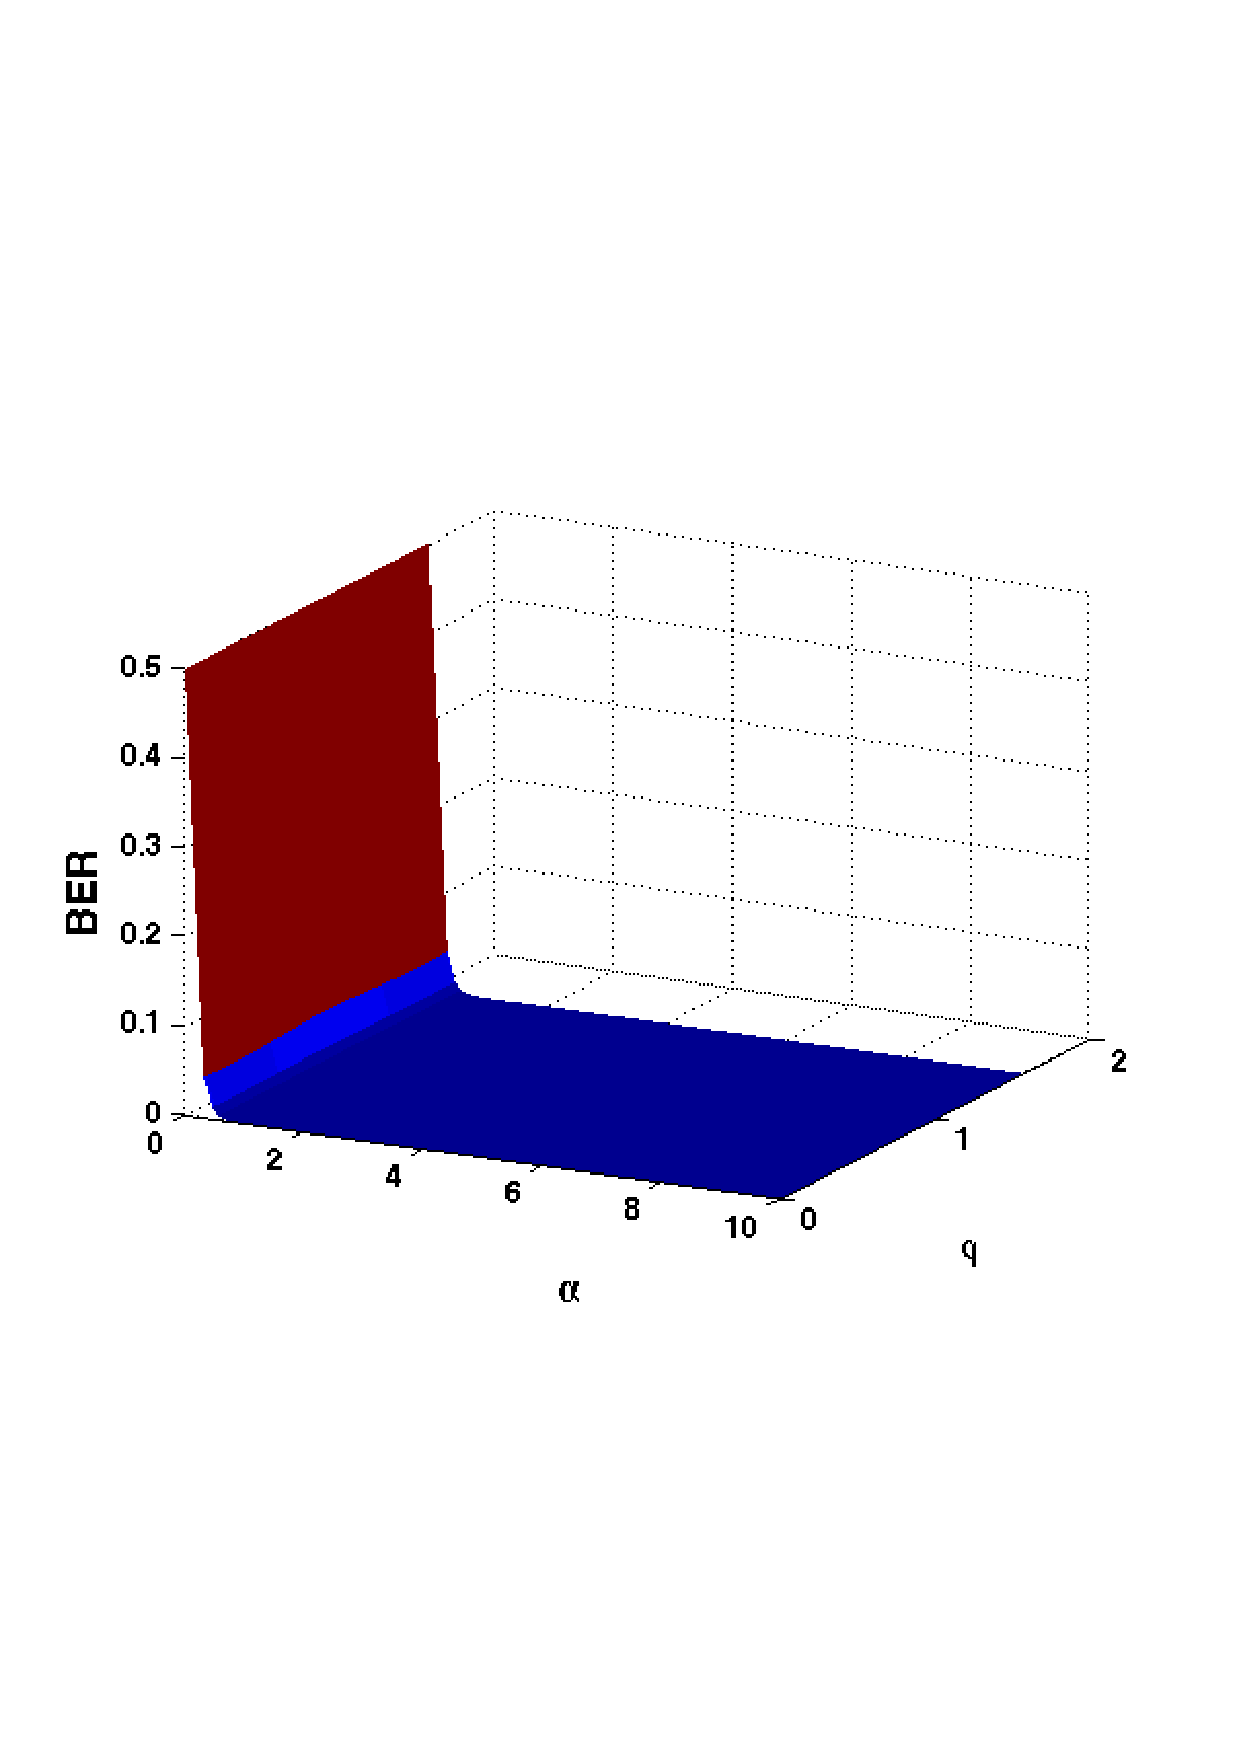
\includegraphics[width=\linewidth, trim= 0mm 60mm 0mm 70mm]{doublehomodyneBER.pdf}
\caption{BER in function of $\alpha$ and $\theta$ for the double homodyne setup. $X_0=1$ was used}
\end{subfigure}
\caption{Theoretical results for double homodyne setup.}
\end{figure}

\subsection*{Functional Description}

Simplified diagrams of the systems being simulated are presented in Figures~\ref{fig:singleH}. and~\ref{fig:doubleH}. Two optical signals are generated, one with a constant power level of 10~dBm and the other with power in multiples of the power corresponding to a single photon per sampling time (6.4078e$\times10^{-13}$~W for a sampling time of 200~ns). The two signals are mixed, with a Balanced Beam Splitter in the single homodyne case and with a 90$^\text{o}$ Optical Hybrid in the double homodyne one, and are subsequently evaluated with recourse to Homodyne Receivers.

\begin{figure}[h]
\centering
\begin{subfigure}{\linewidth}
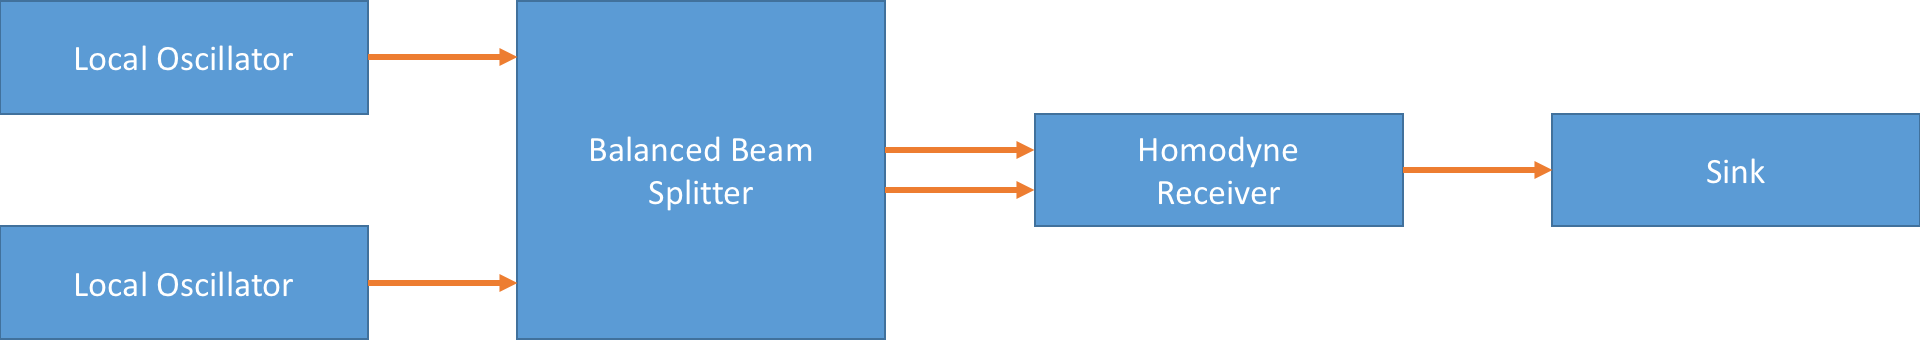
\includegraphics[width=\linewidth]{singlehomodyneSimuBlock.png}
\caption{Single homodyne simulation block diagram.}
\label{fig:singleH}
\end{subfigure}
\\
~
\\
\begin{subfigure}{\linewidth}
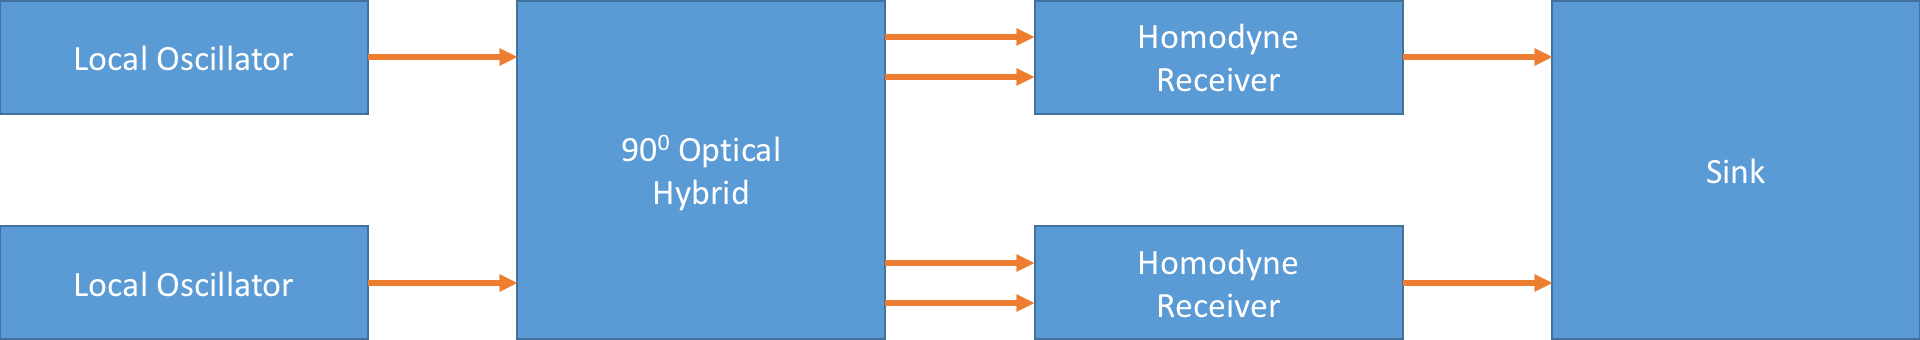
\includegraphics[width=\linewidth]{doublehomodyneSimuBlock.png}
\caption{Double homodyne simulation block diagram.}
\label{fig:doubleH}
\end{subfigure}
\caption{Block diagrams of both simulation results presented in this report.}
\end{figure}

\begin{table}[H]
\centering
\begin{tabular}{c|c}
System Blocks          & netxpto Blocks       \\ \hline
Local Oscillator       & LocalOscillator      \\
Homodyne Receiver      & I\_HomodyneReceiver   \\
Balanced Beam Splitter & BalancedBeamSplitter \\
90$^\text{o}$ Optical Hybrid     & OpticalHybrid
\end{tabular}
\end{table}

\pagebreak
\subsection*{Required files}\label{Required files}

Header Files
\begin{table}[H]
\centering
\begin{tabulary}{1.0\textwidth}{|L|L|}
\hline
\textbf{File}              & \textbf{Description} 				            \\ \hline
netxpto.h                  & Generic purpose simulator definitions.	        \\ \hline
local\_oscillator.h        & Generates continuous coherent signal.            \\ \hline
balanced\_beam\_splitter.h & Mixes the two input signals into two outputs.    \\ \hline
optical\_hybrid.h          & Mixes the two input signals into four outputs.   \\ \hline
homodyne\_reciever.h       & Performs coherent detection on the input signal. \\ \hline
sink.h                     & Closes any unused signals.                       \\ \hline
\end{tabulary}
\end{table}
%
Source Files
\begin{table}[H]
\centering
\begin{tabulary}{1.0\textwidth}{|L|L|}
\hline
\textbf{File}                & \textbf{Description} 					          \\ \hline
netxpto.cpp                  & Generic purpose simulator definitions.	          \\ \hline
local\_oscillator.cpp        & Generates continuous coherent signal.            \\ \hline
balanced\_beam\_splitter.cpp & Mixes the two input signals into two outputs.    \\ \hline
optical\_hybrid.cpp          & Mixes the two input signals into four outputs.   \\ \hline
homodyne\_reciever.cpp       & Performs coherent detection on the input signal. \\ \hline
sink.cpp                     & Closes any unused signals.                       \\ \hline
\end{tabulary}
\end{table}


\subsection*{System Input Parameters}

This system takes into account the following input parameters:
\begin{table}[H]
\centering
\begin{tabulary}{1.0\textwidth}{|C|C|}
\hline
\textbf{System Parameters} & \textbf{Description}                                                                   \\ \hline
numberOfBitsGenerated      & Gives the number of bits to be simulated                                               \\ \hline
bitPeriod                  & Sets the time between adjacent bits                                                    \\ \hline
samplesPerSymbol           & Establishes the number of samples each bit in the string is given                      \\ \hline
localOscillatorPower\_dBm1 & Sets the optical power, in units of dBm, at the reference output	                      \\ \hline
localOscillatorPower2      & Sets the optical power, in units of W, of the signal                                   \\ \hline
localOscillatorPhase1      & Sets the initial phase of the local oscillator used for reference                      \\ \hline
localOscillatorPhase2      & Sets the initial phase of the local oscillator used for signal                         \\ \hline
transferMatrix             & Sets the transfer matrix of the beam splitter used in the homodyne detector            \\ \hline
responsivity               & Sets the responsivity of the photodiodes used in the homodyne detector                 \\ \hline
amplification              & Sets the amplification of the trans-impedance amplifier used in the homodyne detector  \\ \hline
electricalNoiseAmplitude   & Sets the amplitude of the gaussian thermal noise added in the homodyne detector        \\ \hline
shotNoise                  & Chooses if quantum shot noise is used in the simulation                                \\ \hline
\end{tabulary}
\end{table}		

\subsection*{Inputs}

This system takes no inputs.
%
\subsection*{Outputs}

The single homodyne system outputs the following objects:
\begin{itemize}
\item Signals:
\begin{itemize}
\item Local Oscillator Optical Reference; (S$_{1}$)
\item Local Oscillator Optical Signal; (S$_{2}$)
\item Beam Splitter Outputs; (S$_{3}$, S$_{4}$)
\item Homodyne Detector Electrical Output; (S$_{5}$)
\end{itemize}
\end{itemize}
\par
The double homodyne system outputs the following objects:
\begin{itemize}
\item Signals:
\begin{itemize}
\item Local Oscillator Optical Reference; (S$_{1}$)
\item Local Oscillator Optical Signal; (S$_{2}$)
\item 90$^\text{o}$ Optical Hybrid Outputs; (S$_{3}$, S$_{4}$, S$_{5}$, S$_{6}$)
\item Homodyne Detector Electrical Output; (S$_{7}$)
\end{itemize}
\end{itemize}		

\subsection*{Simulation Results}
\subsubsection*{Single homodyne results}\label{subsec:SHresults}

The numerical results presented in Figure~\ref{fig:directber} were obtained with the simulation described by the block diagram in Figure~\ref{fig:singleH}. Theoretical results are a direct trace of~\eqref{eq:biterrorratio}. One can see that the numerical results adhere quite well to the expected curve.

\begin{figure}[h]
\centering
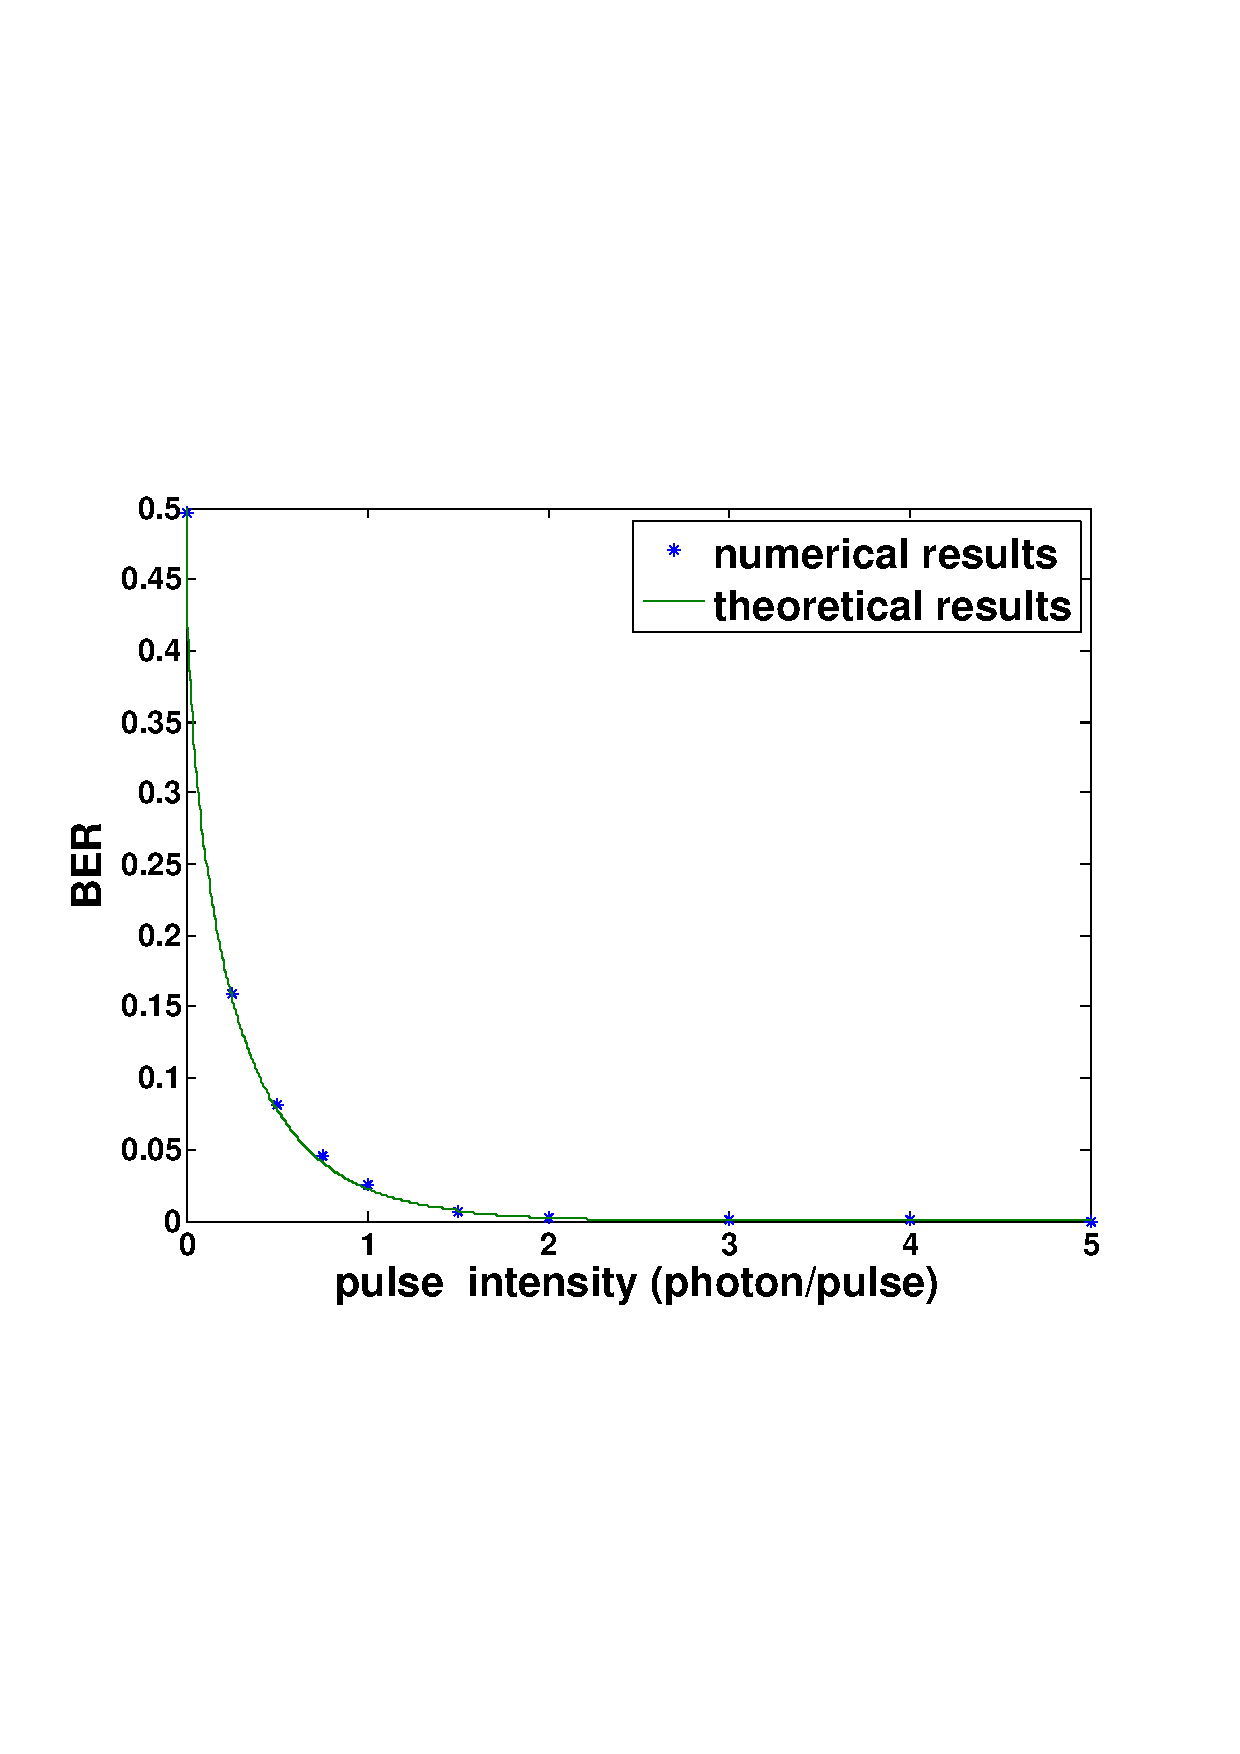
\includegraphics[width=\linewidth, trim= 0mm 60mm 0mm 70mm]{directBER.pdf}
\caption{BER in function of $\alpha$ for the single homodyne setup. $X_0=0$ was used}
\label{fig:directber}
\end{figure}

\subsubsection*{Double homodyne results}\label{subsec:DHresults}

The numerical results presented in Figure~\ref{fig:adaptedber} were obtained with the simulation described by the block diagram in Figure~\ref{fig:doubleH}. Theoretical results are a direct trace of~\eqref{eq:adaptedBER} with $\theta=\frac{\pi}{4}$. One can see that the numerical results adhere quite well to the expected curve.

\begin{figure}[h]
\centering
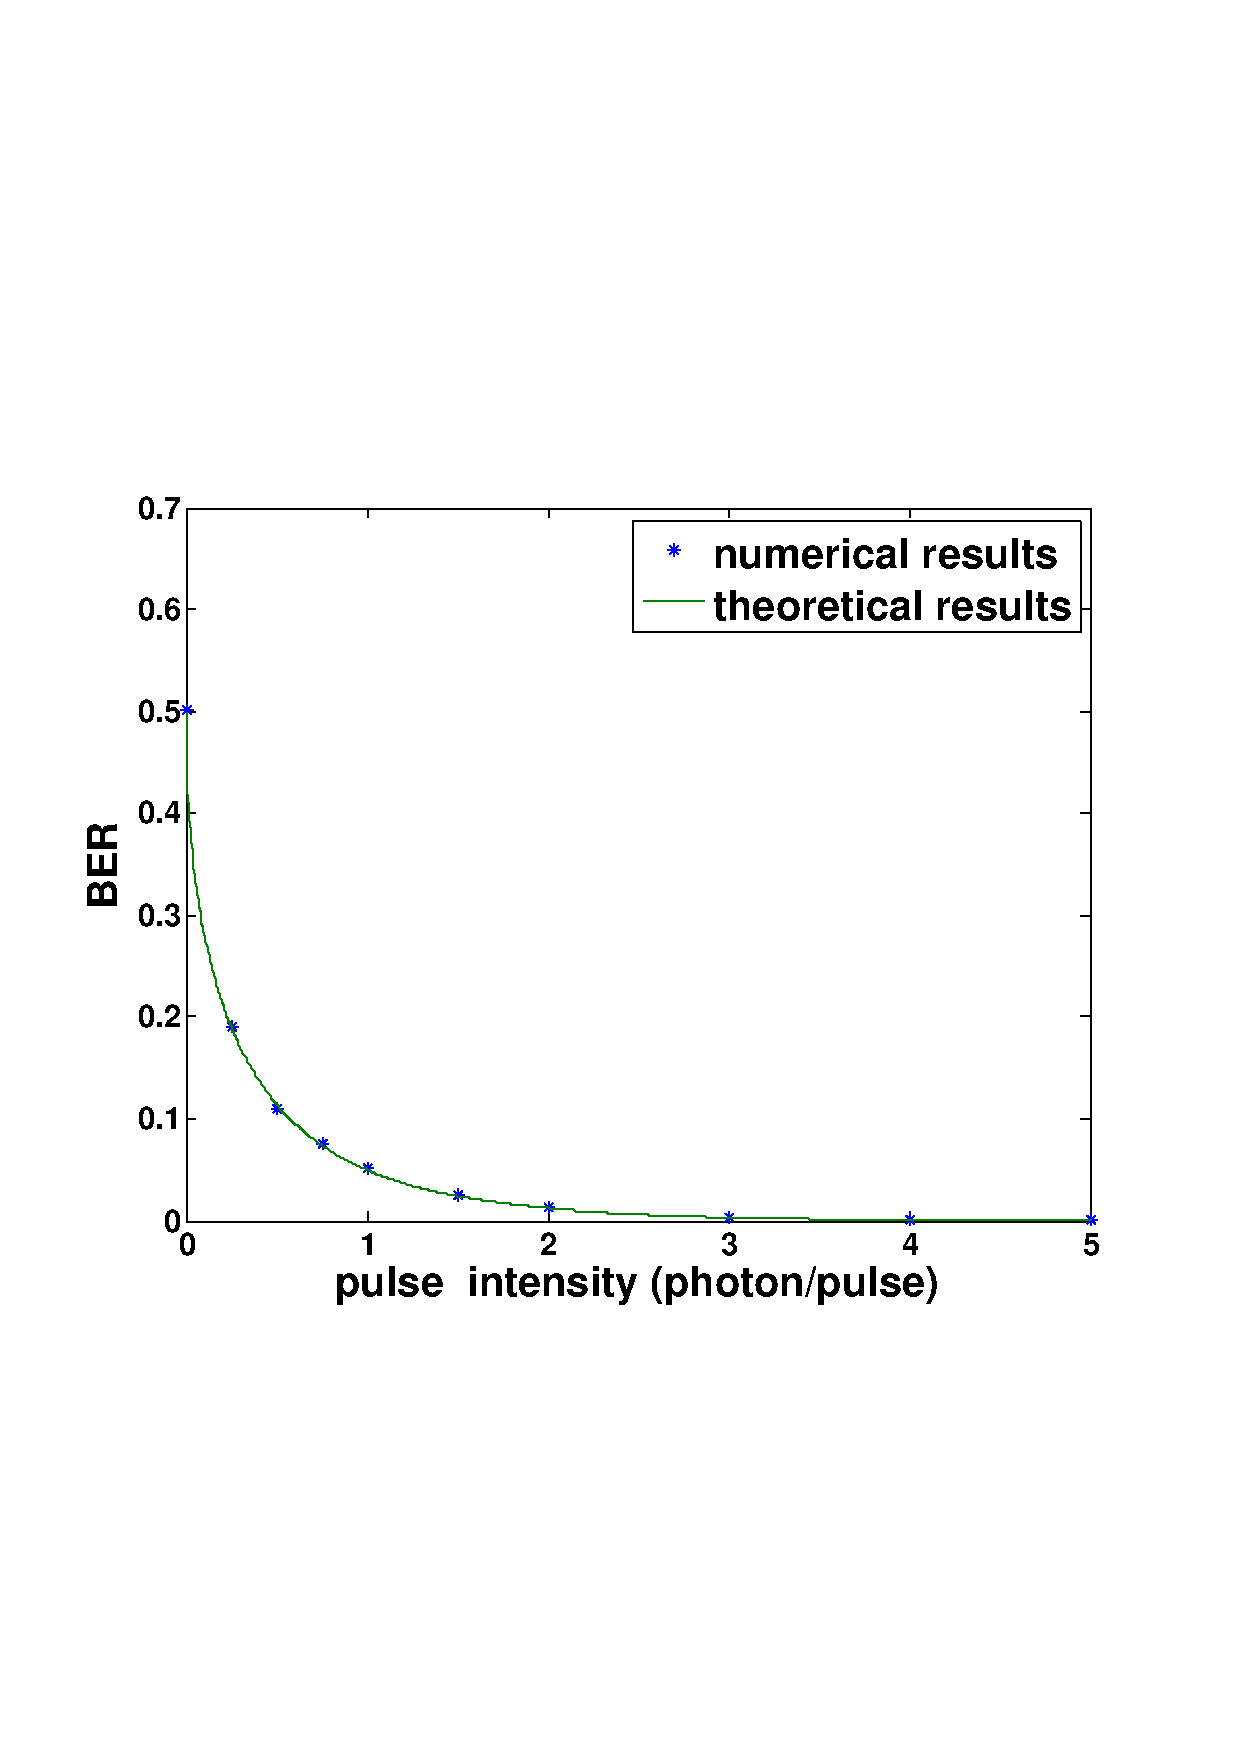
\includegraphics[width=\linewidth, trim= 0mm 60mm 0mm 70mm]{adaptedBER.pdf}
\caption{BER in function of $\alpha$ for the double homodyne setup. $X_0=0$ was used}
\label{fig:adaptedber}
\end{figure}

%\section{Block Description}
%
%\subsection{Homodyne Receiver}
%\subfile{./lib/i_homodyne_receiver}
%
%\subsection{Local Oscillator}
%\subfile{./lib/localoscillator}
%
%\subsection{Beam Splitter}
%\subfile{./lib/beamsplitter}
%
%\subsection{90$^\text{o}$ Optical Hybrid}
%
%\subsection{Photodiode}
%\subfile{./lib/photodiode}
%
%\subsection{Amplifier}
%\subfile{./lib/ideal_amplifier}
%
%\subsection{Electrical Filter}
%\subfile{./lib/pulse_shaper}

\subsection*{Known Problems}
\begin{enumerate}
    \item Homodyne Super-Block not functioning
    \item 90$^\text{o}$ Optical Hybrid PDF needs to be written
\end{enumerate}


\bibliographystyle{unsrt}
\bibliography{bibliography}
%\end{document} 




% ------------------------------------------------------------------------
\chapter{Library}

\clearpage

\section{Add}

\subsection*{Input Parameters}

This block takes no parameters.

\subsection*{Functional Description}

This block accepts two signals and outputs one signal built from a sum of the two inputs. The input and output signals must be of the same type.

\subsection*{Input Signals}

\textbf{Number}: 2

\textbf{Type}: Real, Complex or Complex\_XY signal (ContinuousTimeContinuousAmplitude)

\subsection*{Output Signals}

\textbf{Number}: 1

\textbf{Type}: Real, Complex or Complex\_XY signal (ContinuousTimeContinuousAmplitude)

%\end{document} 
\clearpage

\section{Binary source}

\maketitle
This block generates a sequence of binary values (1 or 0) and it can work in four different modes:

\begin{multicols}{2}
\begin{enumerate}
	\item Random
	\item PseudoRandom
	\item DeterministicCyclic
	\item DeterministicAppendZeros
\end{enumerate}
\end{multicols}

This blocks doesn't accept any input signal. It produces any number of output signals.

\subsection*{Input Parameters}

	\begin{itemize}
		\item mode\{PseudoRandom\}\linebreak
		(Random, PseudoRandom, DeterministicCyclic, DeterministicAppendZeros)
		\item probabilityOfZero\{0.5\}\linebreak
		(real $\in$ [0,1])
		\item patternLength\{7\} \linebreak
		(integer $\in$ [1,32])
		\item bitStream\{"0100011101010101"\} \linebreak
		(string of 0's and 1's)
		\item numberOfBits\{-1\} \linebreak
		(long int)
		\item bitPeriod\{1.0/100e9\} \linebreak
		(double)
	\end{itemize}

\subsection*{Methods}

BinarySource(vector$\langle$Signal *$\rangle$ \&InputSig, vector$\langle$Signal *$\rangle$ \&OutputSig) :Block(InputSig, OutputSig)\{\};
\bigbreak	
void initialize(void);
\bigbreak	
bool runBlock(void);
\bigbreak	
void setMode(BinarySourceMode m)
BinarySourceMode const getMode(void)
\bigbreak	
void setProbabilityOfZero(double pZero)
\bigbreak
double const getProbabilityOfZero(void)
\bigbreak	
void setBitStream(string bStream)
\bigbreak
string const getBitStream(void)
\bigbreak	
void setNumberOfBits(long int nOfBits)
\bigbreak
long int const getNumberOfBits(void)
\bigbreak	
void setPatternLength(int pLength)
\bigbreak
int const getPatternLength(void)
\bigbreak	
void setBitPeriod(double bPeriod)
\bigbreak
double const getBitPeriod(void)

\subsection*{Functional description}

The \textit{mode} parameter allows the user to select between one of the four operation modes of the binary source.

\subparagraph*{Random Mode}
Generates a 0 with probability \textit{probabilityOfZero} and a 1 with probability 1-\textit{probabilityOfZero}.

\subparagraph*{Pseudorandom Mode}
Generates a pseudorandom sequence with period $2^\textit{patternLength}-1$.

\subparagraph*{DeterministicCyclic Mode}
Generates the sequence of 0's and 1's specified by \textit{bitStream} and then repeats it.

\subparagraph*{DeterministicAppendZeros Mode}
Generates the sequence of 0's and 1's specified by \textit{bitStream} and then it fills the rest of the buffer space with zeros.

\subsection*{Input Signals}


\subparagraph*{Number:} 0

\subparagraph*{Type:} Binary (DiscreteTimeDiscreteAmplitude)

\subsection*{Output Signals}

\subparagraph*{Number:} 1 or more

\subparagraph*{Type:} Binary (DiscreteTimeDiscreteAmplitude)

\subsection*{Examples}

\paragraph*{Random Mode}

\paragraph*{PseudoRandom Mode}
As an example consider a pseudorandom sequence with \textit{patternLength}=3 which contains a total of 7 ($2^3-1$) bits. In this sequence it is possible to find every combination of 0's and 1's that compose a 3 bit long subsequence with the exception of $000$. For this example the possible subsequences are $010$, $110$, $101$, $100$, $111$, $001$ and $100$ (they appear in figure \ref{BinarySequenceN3} numbered in this order). Some of these require wrap.

\begin{figure}[h]
	\centering
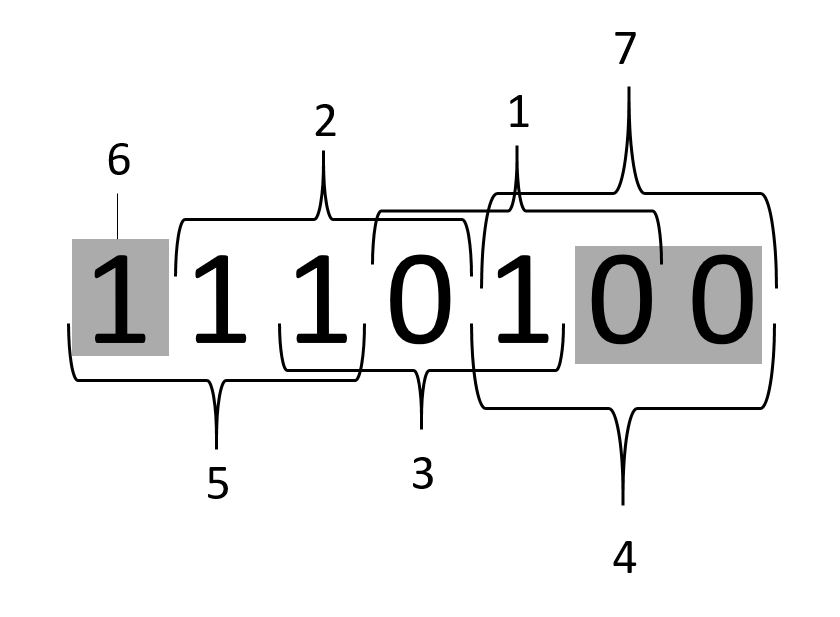
\includegraphics[width=0.5\textwidth]{./lib/binary_source/figures/BinarySequenceN3}
\caption{Example of a pseudorandom sequence with a pattern length equal to 3.}\label{BinarySequenceN3}
\end{figure}

\paragraph*{DeterministicCyclic Mode}

As an example take the \textit{bit stream} '0100011101010101'. The generated binary signal is displayed in.

\paragraph*{DeterministicAppendZeros Mode}

Take as an example the \textit{bit stream} '0100011101010101'. The generated binary signal is displayed in \ref{MQAM1_DeterministAppendZeros}.

\begin{figure}
	\centering
	\includegraphics[width=\textwidth]{./lib/binary_source/figures/BinarySource_output}
	
	\caption{Binary signal generated by the block operating in the \textit{Deterministic Append Zeros} mode with a binary sequence 01000...}\label{MQAM1_DeterministAppendZeros}
\end{figure}

\subsection*{Sugestions for future improvement}

Implement an input signal that can work as trigger.


\clearpage

\section{Clock}

This block doesn't accept any input signal. It outputs one signal that corresponds to a sequence of Dirac's delta functions with a user defined \textit{period}.

\subsection*{Input Parameters}

\begin{itemize}
	\item period\{ 0.0 \};
	\item samplingPeriod\{ 0.0 \};
\end{itemize}

\subsection*{Methods}
 
Clock() {}
\bigbreak
Clock(vector$<$Signal *$>$ \&InputSig, vector$<$Signal *$>$ \&OutputSig) :Block(InputSig, OutputSig) {}
\bigbreak
void initialize(void)
\bigbreak
bool runBlock(void)
\bigbreak
void setClockPeriod(double per)
\bigbreak
void setSamplingPeriod(double sPeriod)

\subsection*{Functional description}


\pagebreak

\subsection*{Input Signals}

\subparagraph*{Number:} 0

\subsection*{Output Signals}

\subparagraph*{Number:} 1

\subparagraph*{Type:} Sequence of Dirac's delta functions. (TimeContinuousAmplitudeContinuousReal)

\subsection*{Examples} 

\begin{figure}[h]
	\centering
	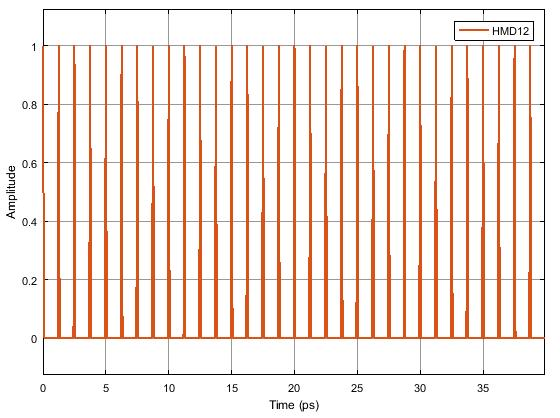
\includegraphics[width=\textwidth]{../homodyne_receiver/figures/Clock_output}
	\caption{Example of the output signal of the clock}\label{Clock_output}
\end{figure}

\subsection*{Sugestions for future improvement}


\clearpage

\section{Decoder}

This block accepts a complex electrical signal and outputs a sequence of binary values (0's and 1's). Each point of the input signal corresponds to a pair of bits.

\subsection*{Input Parameters}

\begin{itemize}
	\item\texttt{t\_integer} m\{ 4 \}
	\item vector$<$\texttt{t\_complex}$>$ iqAmplitudes\{ \{ 1.0, 1.0 \},\{ -1.0, 1.0 \},\{ -1.0, -1.0 \},\{ 1.0, -1.0 \} \};
\end{itemize}

\subsection*{Methods}

Decoder() {}
\bigbreak
Decoder(vector$<$Signal *$>$ \&InputSig, vector$<$Signal *$>$ \&OutputSig) :Block(InputSig, OutputSig) {}
\bigbreak
void initialize(void)
\bigbreak
bool runBlock(void)
\bigbreak
void setM(int mValue)
\bigbreak
void getM()
\bigbreak
void setIqAmplitudes(vector$<$\texttt{t\_iqValues}$>$ iqAmplitudesValues)
\bigbreak
vector$<$\texttt{t\_iqValues}$>$getIqAmplitudes()

\subsection*{Functional description}

This block makes the correspondence between a complex electrical signal and pair of binary values using a predetermined constellation.

To do so it computes the distance in the complex plane between each value of the input signal and each value of the \textit{iqAmplitudes} vector selecting only the shortest one. It then converts the point in the IQ plane to a pair of bits making the correspondence between the input signal and a pair of bits.

\pagebreak

\subsection*{Input Signals}

\subparagraph*{Number:} 1

\subparagraph*{Type:} Electrical complex (TimeContinuousAmplitudeContinuousReal)

\subsection*{Output Signals}

\subparagraph*{Number:} 1

\subparagraph*{Type:} Binary

\subsection*{Examples}

As an example take an input signal with positive real and imaginary parts. It would correspond to the first point of the \textit{iqAmplitudes} vector and therefore it would be associated to the  pair of bits $00$.

\begin{figure}[h]
	\centering
	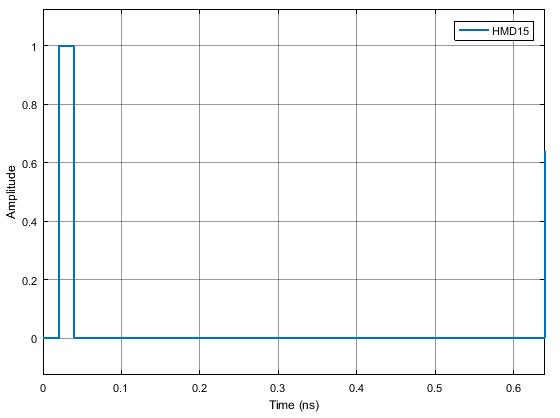
\includegraphics[width=\textwidth]{./lib/decoder/figures/Decoder_output}
	\caption{Example of the output signal of the decoder for a binary sequence 01. As expected it reproduces the initial bit stream}\label{Decoder_output}
\end{figure}

\subsection*{Sugestions for future improvement}

\clearpage

\section{Discrete to continuous time}

This block converts a signal discrete in time to a signal continuous in time. It accepts one input signal that is a sequence of 1's and -1's and it produces one output signal that is a sequence of Dirac delta functions.

\subsection*{Input Parameters}

\begin{itemize}
	\item numberOfSamplesPerSymbol\{8\} \linebreak
	(int)
\end{itemize}

\subsection*{Methods}

DiscreteToContinuousTime(vector$<$Signal *$>$ \&inputSignals, vector$<$Signal *$>$ \&outputSignals) :Block(inputSignals, outputSignals)\{\};
\bigbreak	
void initialize(void);
\bigbreak	
bool runBlock(void);
\bigbreak	
void setNumberOfSamplesPerSymbol(int nSamplesPerSymbol)
\bigbreak
int const getNumberOfSamplesPerSymbol(void)

\subsection*{Functional Description}

This block reads the input signal buffer value, puts it in the output signal buffer and it fills the rest of the space available for that symbol with zeros. The space available in the buffer for each symbol is given by the parameter \textit{numberOfSamplesPerSymbol}.

\subsection*{Input Signals}

\subparagraph*{Number}: 1

\subparagraph*{Type}: Sequence of 1's and -1's. (DiscreteTimeDiscreteAmplitude)

\subsection*{Output Signals}

\subparagraph*{Number}: 1

\subparagraph*{Type}: Sequence of Dirac delta functions (ContinuousTimeDiscreteAmplitude)

\subsection*{Example}

\begin{figure}[h]
	\centering
	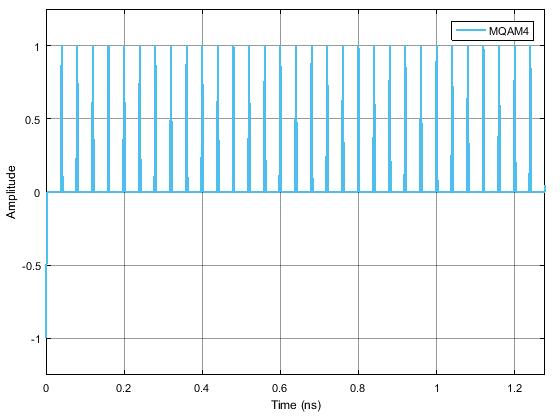
\includegraphics[width=\textwidth]{../lib/discrete_to_continuous_time/figures/TimeDiscreteToContinuous_output}
	\label{MQAM4_DeterministicAppendZeros}\caption{Example of the type of signal generated by this block for a binary sequence 0100...}
\end{figure}

%\subsection*{Sugestions for future improvement}

\pagebreak

\clearpage

\section{Homodyne receiver}

This block of code simulates the reception and demodulation of an optical signal (which is the input signal of the system) outputing a binary signal. A simplified schematic representation of this block is shown in figure \ref{MQAM_receiver_block_diagram_simple}.

\begin{figure}[h]
	\centering
	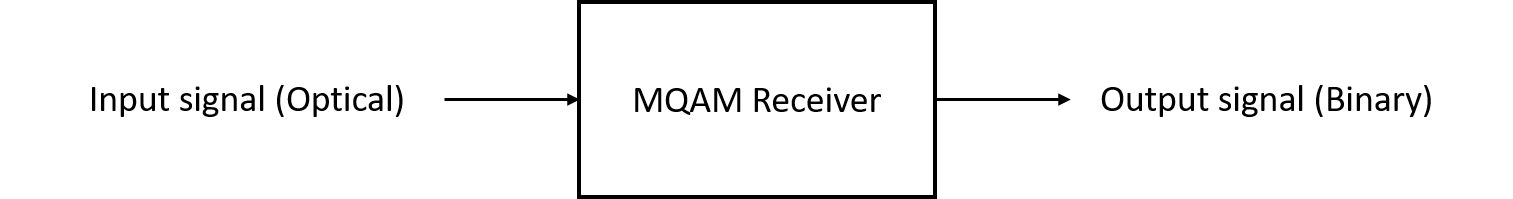
\includegraphics[width=0.8\textwidth]{../lib/homodyne_receiver/figures/MQAM_receiver_block_diagram_simple}
	\caption{Basic configuration of the MQAM receiver}\label{MQAM_receiver_block_diagram_simple}
\end{figure}

\subsection*{Functional description}

This block accepts one optical input signal and outputs one binary signal that corresponds to the M-QAM demodulation of the input signal. It is a complex block (as it can be seen from figure \ref{MQAM_receiver_block_diagram}) of code made up of several simpler blocks whose description can be found in the \textit{lib} repository.

In can also be seen from figure \ref{MQAM_receiver_block_diagram} that there's an extra internal (generated inside the homodyne receiver block) input signal generated by the \textit{Clock}. This block is used to provide the sampling frequency to the \textit{Sampler}.


\begin{figure}[h]
	\centering
	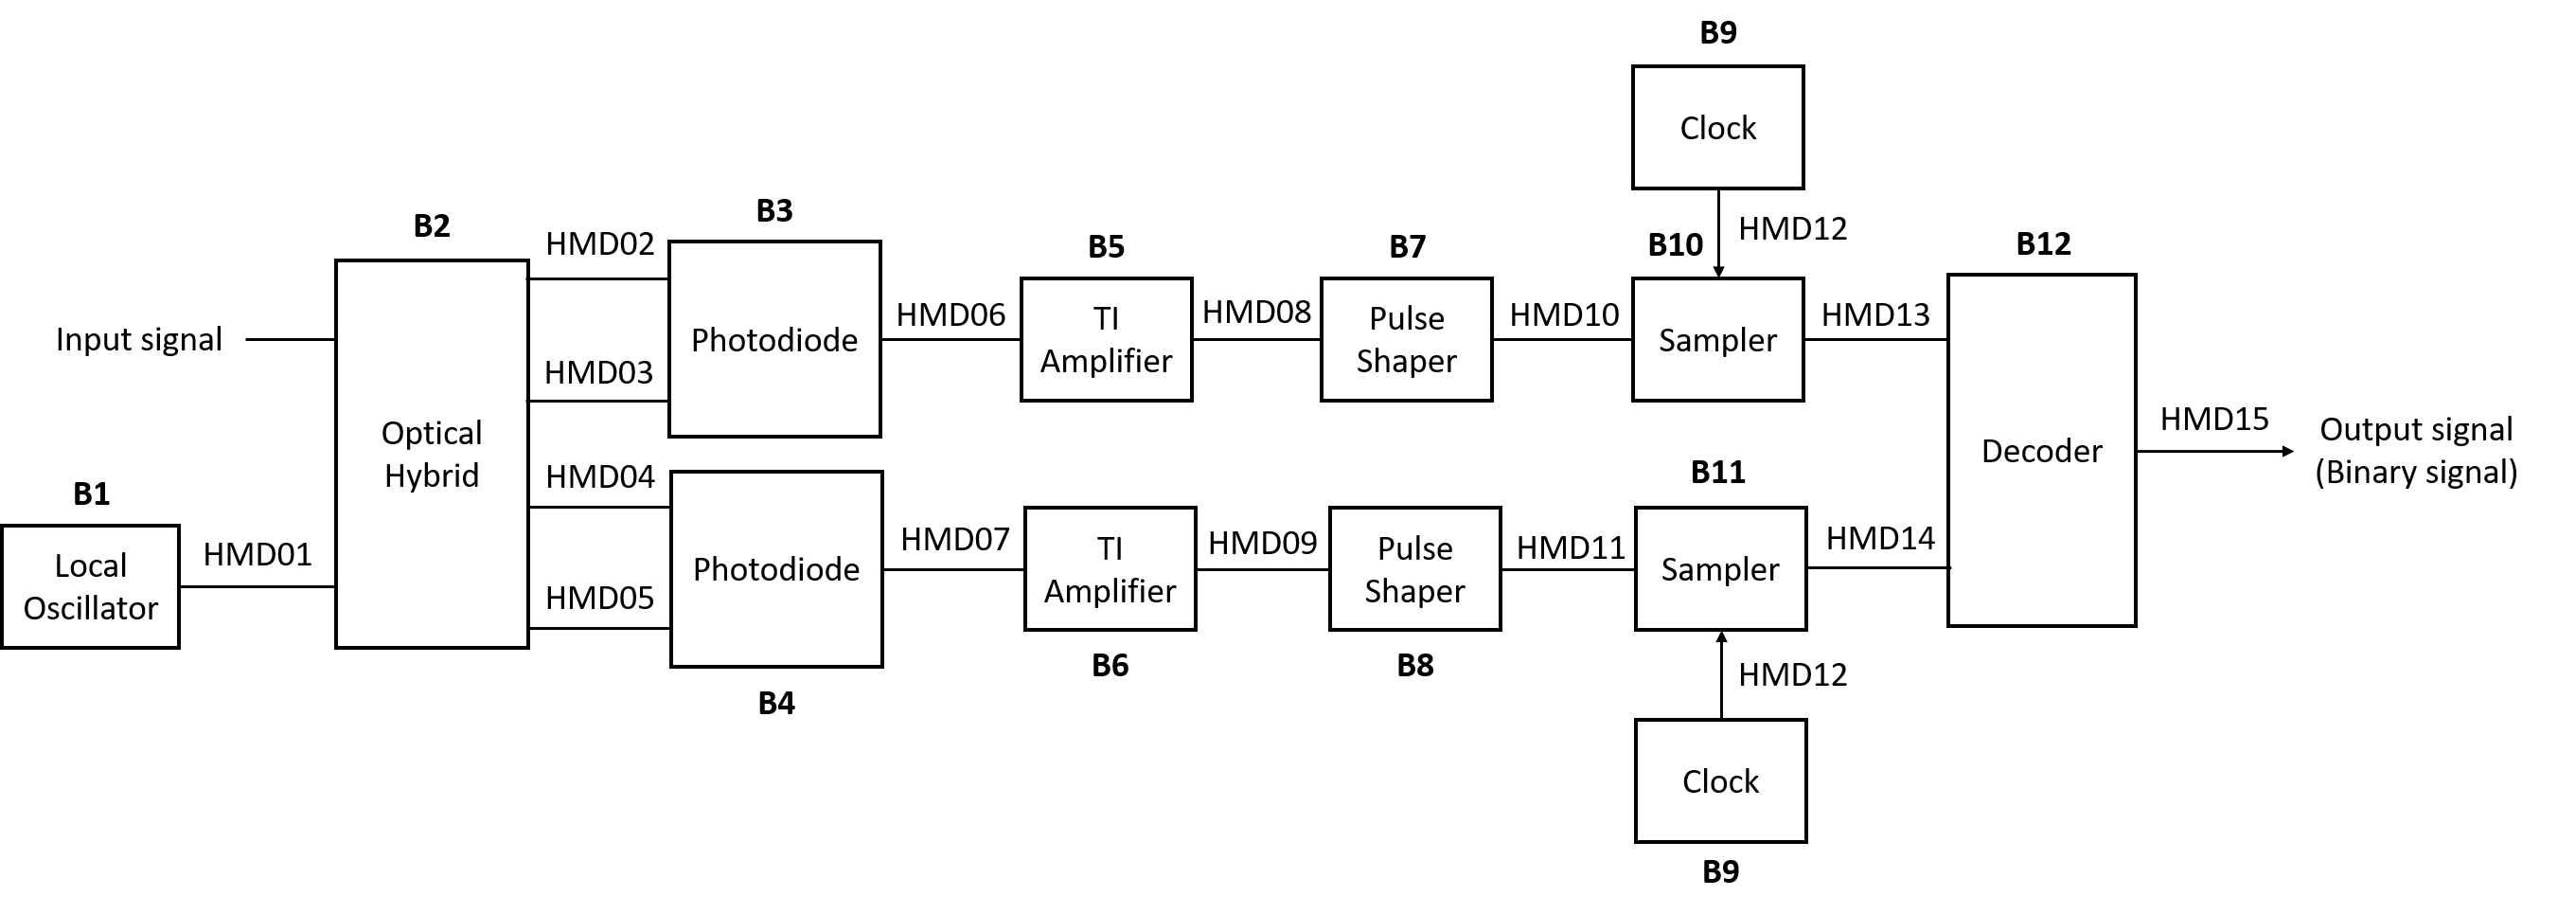
\includegraphics[width=\textwidth]{../lib/homodyne_receiver/figures/MQAM_receiver_block_diagram}
	\caption{Schematic representation of the block homodyne receiver.}\label{MQAM_receiver_block_diagram}
\end{figure}

\subsection*{Input parameters}

This block has some input parameters that can be manipulated by the user in order oto change the basic configuration of the receiver. Each parameter has associated a function that allows for its change. In the following table (table~\ref{table}) the input parameters and corresponding functions are summarized.

\begin{table}[h]
	\begin{center}
		\begin{tabular}{| m{3,5cm} | m{5,8cm} |  m{2,5cm} | m{4cm} | }
			\hline
			\textbf{Input parameters} & \textbf{Function} & Type & \textbf{Accepted values} \\ \hline
			IQ amplitudes & setIqAmplitudes & Vector of coordinate points in the I-Q plane & \textbf{Example} for a 4-qam mapping: \{ \{ 1.0, 1.0 \}, \{ -1.0, 1.0 \}, \{ -1.0, -1.0 \}, \{ 1.0, -1.0 \} \} \\ \hline
			Local oscillator power (in dBm) & setLocalOscillatorOpticalPower\_dBm & double(t\_real) & Any double greater than zero\\ \hline
			Local oscillator phase & setLocalOscillatorPhase & double(t\_real) & Any double greater than zero\\ \hline
			Responsivity of the photodiodes & setResponsivity & double(t\_real) &$\in$ [0,1] \\ \hline
			Amplification (of the TI amplifier) & setAmplification & double(t\_real) & Positive real number\\ \hline
			Noise amplitude (introduced by the TI amplifier) & setNoiseAmplitude & double(t\_real) & Real number greater than zero \\ \hline
			Samples to skipe & setSamplesToSkip & int(t\_integer) &  \\ \hline
			Save internal signals & setSaveInternalSignals & bool & True or False\\ \hline
			Sampling period & setSamplingPeriod & double & Givem by \textit{symbolPeriod}/\textit{samplesPerSymbol}\\
			\hline
		\end{tabular}
		\caption{List of input parameters of the block MQAM receiver} \label{table}
	\end{center}
\end{table}

\pagebreak

\subsection*{Methods}

HomodyneReceiver(vector$<$Signal *$>$ \&inputSignal, vector$<$Signal *$>$ \&outputSignal) (\textbf{constructor})
\bigbreak
void setIqAmplitudes(vector$<$t\_iqValues$>$ iqAmplitudesValues)
\bigbreak
vector$<$t\_iqValues$>$ const getIqAmplitudes(void)
\bigbreak
void setLocalOscillatorSamplingPeriod(double sPeriod)
\bigbreak
void setLocalOscillatorOpticalPower(double opticalPower)
\bigbreak
void setLocalOscillatorOpticalPower\_dBm(double opticalPower\_dBm)
\bigbreak
void setLocalOscillatorPhase(double lOscillatorPhase)
\bigbreak
void setLocalOscillatorOpticalWavelength(double lOscillatorWavelength)
\bigbreak
void setSamplingPeriod(double sPeriod)
\bigbreak
void  setResponsivity(t\_real Responsivity)
\bigbreak
void setAmplification(t\_real Amplification)
\bigbreak
void setNoiseAmplitude(t\_real NoiseAmplitude)
\bigbreak
void setImpulseResponseTimeLength(int impResponseTimeLength)
\bigbreak
void setFilterType(PulseShaperFilter fType)
\bigbreak
void setRollOffFactor(double rOffFactor)
\bigbreak
void setClockPeriod(double per)
\bigbreak
void setSamplesToSkip(int sToSkip)

\pagebreak

\subsection*{Input Signals}

\subparagraph*{Number:} 1

\subparagraph*{Type:} Optical signal

\subsection*{Output Signals}

\subparagraph*{Number:} 1

\subparagraph*{Type:} Binary signal

\subsection*{Example}

\subsection*{Sugestions for future improvement}

\clearpage

\section{IQ modulator}

This blocks accepts one inupt signal continuous in both time and amplitude and it can produce either one or two output signals. It generates an optical signal and it can also generate a binary signal. 

\subsection*{Input Parameters}

\begin{itemize}
	\item outputOpticalPower\{1e-3\} \linebreak
	(double)
	\item outputOpticalWavelength\{1550e-9\} \linebreak (double)
	\item outputOpticalFrequency\{speed$\_$of$\_$light/outputOpticalWavelength\} \linebreak
	(double)
\end{itemize}

\subsection*{Methods}

IqModulator(vector$<$Signal *$>$ \&InputSig, vector$<$Signal *$>$ \&OutputSig) :Block(InputSig, OutputSig)\{\};
\bigbreak
void initialize(void);
\bigbreak
bool runBlock(void);
\bigbreak
void setOutputOpticalPower(double outOpticalPower) 
\bigbreak
void setOutputOpticalPower$\_$dBm(double outOpticalPower$\_$dBm) 
\bigbreak
void setOutputOpticalWavelength(double outOpticalWavelength) 
\bigbreak
void setOutputOpticalFrequency(double outOpticalFrequency) 

\subsection*{Functional Description}

This block takes the two parts of the signal: in phase and in amplitude and it combines them to produce a complex signal that contains information about the amplitude and the phase.

This complex signal is multiplied by $\frac{1}{2}\sqrt{\textit{outputOpticalPower}}$ in order to reintroduce the information about the energy (or power) of the signal. This signal corresponds to an optical signal and it can be a scalar or have two polarizations along perpendicular axis. It is the signal that is transmited to the receptor. 

The binary signal is sent to the Bit Error Rate (BER) meaurement block.

\subsection*{Input Signals}

\subparagraph*{Number}: 2

\subparagraph*{Type}: Sequence of impulses modulated by the filter (ContinuousTimeContiousAmplitude))

\subsection*{Output Signals}

\subparagraph*{Number}: 1 or 2

\subparagraph*{Type}: Complex signal (optical) (ContinuousTimeContinuousAmplitude) and binary signal (DiscreteTimeDiscreteAmplitude)

\subsection*{Example}
\begin{figure}[h]
	\centering
	\includegraphics[width=\textwidth]{../m_qam_transmitter/figures/IQmodulator0_output}
	\label{MQAM8_DeterministicAppendZeros}\caption{Example of a signal generated by this block for the initial binary signal 0100...}
\end{figure}

%\subsection*{Sugestions for future improvement}

\clearpage

\section{Local Oscillator}

This block simulates a local oscillator which can have shot noise or not. It produces one output complex signal and it doesn't accept input signals.

\subsection*{Input Parameters}

\begin{itemize}
	\item opticalPower\{ 1e-3 \}
	\item wavelength\{ 1550e-9 \}
	\item frequency\{ SPEED\_OF\_LIGHT / wavelength \}
	\item phase\{ 0 \}
	\item samplingPeriod\{ 0.0 \}
	\item shotNoise\{ false \}
\end{itemize}

\subsection*{Methods}

LocalOscillator() {}
\bigbreak
LocalOscillator(vector$<$Signal *$>$ \&InputSig, vector$<$Signal *$>$ \&OutputSig) :Block(InputSig, OutputSig)\{\};
\bigbreak
void initialize(void);
\bigbreak
bool runBlock(void);
\bigbreak
void setSamplingPeriod(double sPeriod);
\bigbreak
void setOpticalPower(double oPower);
\bigbreak
void setOpticalPower\_dBm(double oPower\_dBm);
\bigbreak
void setWavelength(double wlength);
\bigbreak
void setPhase(double lOscillatorPhase);
\bigbreak
void setShotNoise(bool sNoise);

\subsection*{Functional description}

This block generates a complex signal with a specified phase given by the input parameter \textit{phase}.

It can have shot noise or not which corresponds to setting the \textit{shotNoise} parameter to True or False, respectively. If there isn't shot noise the the output of this block is given by $0.5*\sqrt{OpticalPower}*ComplexSignal$. If there's shot noise then a random gaussian distributed noise component is added to the \textit{OpticalPower}.

\pagebreak
\subsection*{Input Signals}

\subparagraph*{Number:} 0

\subsection*{Output Signals}

\subparagraph*{Number:} 1

\subparagraph*{Type:} Optical signal

\subsection*{Examples}

\subsection*{Sugestions for future improvement}



\documentclass[a4paper]{article}
\usepackage[top=1in, bottom=1.25in, left=1.25in, right=1.25in]{geometry}
\usepackage{amsmath}
\usepackage{multicol}
\usepackage{graphicx}
\RequirePackage{ltxcmds}[2010/12/07]
%opening
\title{M-QAM Mapper}

\begin{document}
	
\maketitle

This block does the mapping of the binary signal using a \textit{m}-QAM modulation. It atributes to each pair of bits a point in the I-Q space. The constellation is defined by the \textit{iqAmplitudes} vector.

\subsection*{Input Parameters}

\begin{itemize}
	\item m 
	\item iqAmplitudes 
\end{itemize}

\subsection*{Functional Description}



\subsection*{Input Signals}

\textbf{Number}: 1

\textbf{Type}: Binary (DiscreteTimeDiscreteAmplitude)

\subsection*{Output Signals}

\textbf{Number}: 2

\textbf{Type}: Sequence of 1's and -1's (DiscreteTimeDiscreteAmplitude)

\subsection*{Examples}

\begin{figure}[h]
	\includegraphics[width=\textwidth]{MQAM2}
\end{figure}

\subsection*{Sugestions for future improvement}

\end{document}
\clearpage 

\section{MQAM transmitter}

This block generates a MQAM optical signal. It can also output the binary sequence. A schematic representation of this block is shown in figure \ref{MQAM_transmitter_block_diagram_simple}.

\begin{figure}[h]
	\centering
	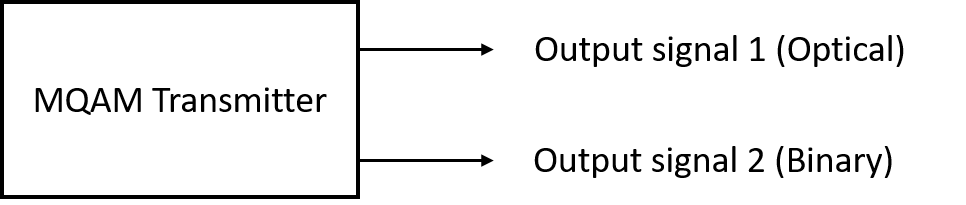
\includegraphics[width=0.5\textwidth]{figures/MQAM_transmitter_block_diagram_simple}
	\caption{Basic configuration of the MQAM transmitter}\label{MQAM_transmitter_block_diagram_simple}
\end{figure}

\subsection*{Functional description}

This block generates an optical signal (output signal 1 in figure \ref{MQAM_transmitter_block_diagram}). The binary signal generated in the internal block Binary Source (block B1 in figure \ref{MQAM_transmitter_block_diagram}) can be used to perform a Bit Error Rate (BER) measurement and in that sense it works as an extra output signal (output signal 2 in figure \ref{MQAM_transmitter_block_diagram}).

\begin{figure}[h]
	\centering
	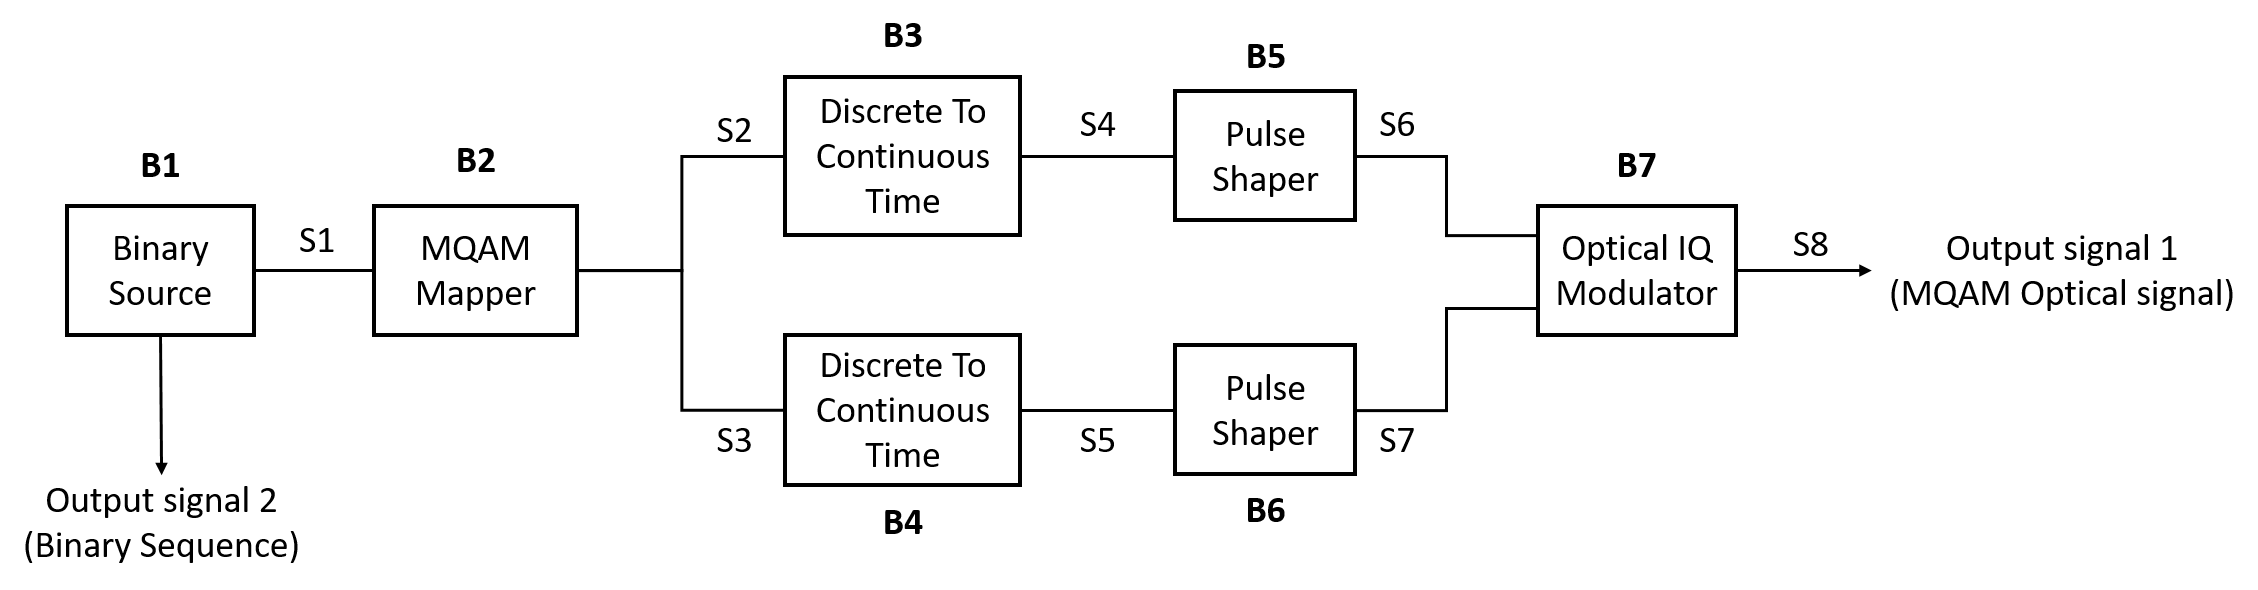
\includegraphics[width=\textwidth]{figures/MQAM_transmitter_block_diagram}
	\caption{Schematic representation of the block MQAM transmitter.}\label{MQAM_transmitter_block_diagram}
\end{figure}

\subsection*{Input parameters}

This block has a special set of functions that allow the user to change the basic configuration of the transmitter. The list of input parameters, functions used to change them and the values that each one can take are summarized in table \ref{table}.

\begin{table}[h]
\begin{center}
	\begin{tabular}{| m{3,5cm} | m{5,1cm} |  m{2,5cm} | m{4cm} | }
		\hline 
		\textbf{Input parameters} & \textbf{Function} & Type & \textbf{Accepted values} \\ \hline
		Mode & setMode() & string & PseudoRandom \newline Random \newline DeterministicAppendZeros \newline DeterministicCyclic \\ \hline
		Number of bits generated & setNumberOfBits() & int & Any integer\\ \hline
		Pattern length & setPatternLength() & int & Real number greater than zero\\ \hline
		Number of bits & setNumberOfBits() & long & Integer number greater than zero\\ \hline
		Number of samples per symbol & setNumberOfSamplesPerSymbol() & int & Integer number of the type $2^n$ with n also integer\\ \hline
		Roll of factor & setRollOfFactor() & double & $\in$ [0,1] \\ \hline
		IQ amplitudes & setIqAmplitudes() & Vector of coordinate points in the I-Q plane & \textbf{Example} for a 4-qam mapping: \{ \{ 1.0, 1.0 \}, \{ -1.0, 1.0 \}, \{ -1.0, -1.0 \}, \{ 1.0, -1.0 \} \} \\ \hline
		Output optical power & setOutputOpticalPower() & int & Real number greater than zero\\ \hline
		Save internal signals & setSaveInternalSignals() & bool & True or False\\
		\hline
	\end{tabular}
	\caption{List of input parameters of the block MQAM transmitter} \label{table} 
\end{center}
\end{table}

%\begin{itemize}
%	\item setMode(PseudoRandom);
%	\item setBitPeriod(1.0/50e9);
%	\linebreak (double)
%	\item setPatternLength(3);
%	\linebreak (int)
%	\item setNumberOfBits(10000);
%	\linebreak (long)
%	\item setNumberOfSamplesPerSymbol(32);
%	\linebreak (int)
%	\item setRollOffFactor(0.9);
%	\linebreak (double $\in$ [0,1])
%	\item setIqAmplitudes(\{ \{ 1, 1 \}, \{ -1, 1 \}, \{ -1, -1 \}, \{ 1, -1 \} \});
%	\item setOutputOpticalPower\_dBm(0);
%	\item setSaveInternalSignals(true);
%\end{itemize}

\pagebreak

\subsection*{Methods}

MQamTransmitter(vector$<$Signal *$>$ \&inputSignal, vector$<$Signal *$>$ \&outputSignal); (\textbf{constructor})
\bigbreak

void set(int opt);
\bigbreak
void setMode(BinarySourceMode m)
\bigbreak
BinarySourceMode const getMode(void)
\bigbreak
void setProbabilityOfZero(double pZero)
\bigbreak
double const getProbabilityOfZero(void)
\bigbreak
void setBitStream(string bStream) 
\bigbreak
string const getBitStream(void)
\bigbreak
void setNumberOfBits(long int nOfBits)
\bigbreak
long int const getNumberOfBits(void)
\bigbreak
void setPatternLength(int pLength) 
\bigbreak
int const getPatternLength(void) 
\bigbreak
void setBitPeriod(double bPeriod) 
\bigbreak
double const getBitPeriod(void) 
\bigbreak
void setM(int mValue)
int const getM(void) 
\bigbreak
void setIqAmplitudes(vector$<$t\textunderscore iqValues$>$ iqAmplitudesValues) 
\bigbreak
vector$<$t\textunderscore iqValues$>$ const getIqAmplitudes(void)
\bigbreak
void setNumberOfSamplesPerSymbol(int n)
\bigbreak
int const getNumberOfSamplesPerSymbol(void)
\bigbreak
void setRollOffFactor(double rOffFactor)
\bigbreak
double const getRollOffFactor(void)
\bigbreak
void setSeeBeginningOfImpulseResponse(bool sBeginningOfImpulseResponse)
\bigbreak
double const getSeeBeginningOfImpulseResponse(void)
\bigbreak
void setOutputOpticalPower(t\textunderscore real outOpticalPower)
\bigbreak
t\textunderscore real const getOutputOpticalPower(void)
\bigbreak
void setOutputOpticalPower\_dBm(t\_real outOpticalPower\_dBm) 
\bigbreak
t\_real const getOutputOpticalPower\_dBm(void)
\pagebreak

\subsection*{Output Signals}

\subparagraph*{Number:} 1 optical and 1 binary (optional)

\subparagraph*{Type:} Optical signal

\subsection*{Example} 

\begin{figure}[h]
	\centering
	\includegraphics[width=0.8\textwidth]{figures/BinarySource_output}
	\caption{Example of the binary sequence generated by this block for a sequence 0100...}
\end{figure}

\begin{figure}[h]
	\centering
	\includegraphics[width=0.8\textwidth]{figures/IQmodulator0_output}
	\caption{Example of the output optical signal generated by this block for a sequence 0100...}
\end{figure}

\subsection*{Sugestions for future improvement}

Add to the system another block similar to this one in order to generate two optical signals with perpendicular polarizations. This would allow to combine the two optical signals and generate an optical signal with any type of polarization.






%\section{Continuous Variable Quantum Transmission System}
%
%\subfile{./sdf/cv_system/cv_system}


%%\documentclass[a4paper]{article}
%
%% subfile handling packages
%\usepackage{subfiles}
%\newcommand{\onlyinsubfile}[1]{#1}
%\newcommand{\notinsubfile}[1]{}
%
%% document packages
%\usepackage[top=1in, bottom=1.25in, left=1.25in, right=1.25in]{geometry}
%\usepackage{amsmath}
%\usepackage{multicol}
%\usepackage{caption}
%\usepackage{subcaption}
%\usepackage{graphicx}
%\usepackage{multirow}
%\usepackage{tabulary}
%\usepackage{hhline}
%\usepackage{indentfirst}
%\RequirePackage{ltxcmds}[2010/12/07]
%\graphicspath{{../../images/}}
%%\graphicspath
%\usepackage{float}
%\usepackage{amsfonts}
%\usepackage{hyperref}
%\usepackage{footnote}
%\makesavenoteenv{tabular}
%\usepackage{braket}
%%opening
%\title{Safety study}
%\author{}
%\date{}
%
%
%\begin{document}
%\maketitle
\clearpage
\section{Continuos Variable Quantum Transmission System}\label{sec:intro}

In this section a continuous varible quantum transmission system is analyzed.
The results here presented follow closely the~\cite{namiki2003security}.
In~\cite{namiki2003security}, the security of a continuous variable quantum key distribution (CV-QKD) system is studied theoretically, here we complete that theoretical study with simulations results.

\begin{figure}[h]
\centering
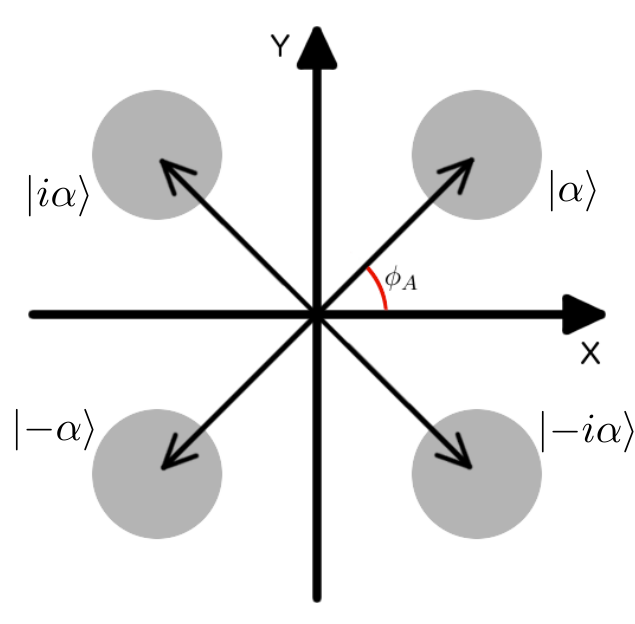
\includegraphics[width=.5\linewidth]{./sdf/cv_system/figures/constellation.png}
\caption{State constellation}
\label{fig:const}
\end{figure}

The state constellation used in the system is presented in Figure~\ref{fig:const}.
The emitter (usually named Alice) is going to use two basis, the $45º$ base and the $-45º$ base.
In the $45º$ base, Alice sends one of two values, $1$ and $-1$, which correspond to the states $\ket{\alpha}$ and $\ket{-\alpha}$.
In the $-45º$ base, Alice can also send one of two values, $1$ and $-1$, which correspond to the states $\ket{-i\alpha}$ and $\ket{i\alpha}$.
At the end Alice is going to send one of the four states $\ket{\alpha}$, $\ket{-\alpha}$, $\ket{-i\alpha}$, and $\ket{i\alpha}$, with equal probability.

Because we don't know $\grave{a}$ prior which state is going be transmitted, neither which basis is going to be used, and to incorporate our ``ignorance"\, in the system description, we can work with the density operator. The density operator is a proper tool to describe ``statistical mixtures". A ``statistical mixtures" is one state, from a possible set, but we don't know which state it is. There is no state superposition.

Since all states have the same probability of occurring, the state density operator is given by:

\begin{equation}\label{eq:statedensity}
\hat{\rho}=\frac{1}{4}\left(\ket{\alpha}\bra{\alpha}+\ket{-\alpha}\bra{-\alpha}+\ket{i\alpha}\bra{i\alpha}+\ket{-i\alpha}\bra{-i\alpha}\right).
\end{equation}

The probability to detect at the receiver the state $\ket{\alpha}$ is given by
\begin{equation}\label{eq:statedensity}
P(\alpha)=\bra{\alpha}\hat{\rho}\ket{\alpha}=\frac{1}{4}.
\end{equation}


Note that the density operator is equivalent to the wave function in terms of the system description.

From the receiver perspective, i.e. from the Bob perspective, and after knowing the base used by Alice.
The density operator can be reduce to,

\begin{align}
\hat{\rho}_1&=\frac{1}{2}\left(\ket{\alpha}\bra{\alpha}+\ket{-\alpha}\bra{-\alpha}\right),\label{eq:statedensity1} \\
\hat{\rho}_2&=\frac{1}{2}\left(\ket{i\alpha}\bra{i\alpha}+\ket{-i\alpha}\bra{-i\alpha}\right).\label{eq:statedensity2}
\end{align}

where $1$ corresponds to the $45º$ base and $-1$ corresponds to $-45º$.

\subsubsection*{Single Base Homodyne Detection}


The probability of obtaining a quadrature $\hat{X}_\phi=\hat{X}_1\cos\phi+\hat{X}_2\sin\phi$ when measuring the coherent state $\ket{\alpha}$ is given by the following gaussian distribution:

\begin{equation}
\left|\braket{X_\phi|\alpha}\right|^2=\sqrt{\frac{2}{\pi}}e^{-2(X_\phi-\alpha\cos\phi)^2},
\end{equation}

We can define the "correct" and "wrong" basis measurement probability density, respectively, as:

\begin{equation}\label{eq:probdensity}
\bra{X_i}\hat{\rho}_j\ket{X_i}=
\begin{cases}
\frac{1}{\sqrt{2\pi}}\left(e^{-2(X_i-\alpha)^2}+e^{-2(X_i+\alpha)}\right), & i=j\\
\sqrt{\frac{2}{\pi}}e^{-2X_i^2}, &i\neq j
\end{cases}.
\end{equation}

The post selection efficiency (PSE) can be defined as the probability of a measurement in the correct basis yields a result that satisfies the limit value $X_0$:

\begin{equation}\label{eq:postselecteff}
\begin{aligned}
P(X_0,\alpha)&=\int^{-X_0}_{-\infty}\bra{X_1}\hat{\rho}_1\ket{X_1}dX_1+\int^{\infty}_{X_0}\bra{X_1}\hat{\rho}_1\ket{X_1}dX_1\\
&=\frac{1}{2}\left[\text{erfc}(\sqrt{2}(X_0+\alpha))+\text{erfc}(\sqrt{2}(X_0-\alpha))\right].
\end{aligned}
\end{equation}

The bit error rate (BER) is the normalized probability of, after choosing the correct basis, obtaining the wrong bit value:

\begin{equation}\label{eq:biterrorratio}
Q(X_0,\alpha)=\frac{1}{P(X_0,\alpha)}\int_{-\infty}^{-X_0}\left|\braket{X_i|\alpha}\right|dX_i=\frac{\text{erfc}\left(\sqrt{2}(X_0+\alpha)\right)}{2P(X_0,n)}
\end{equation}

\begin{figure}[h]
\centering
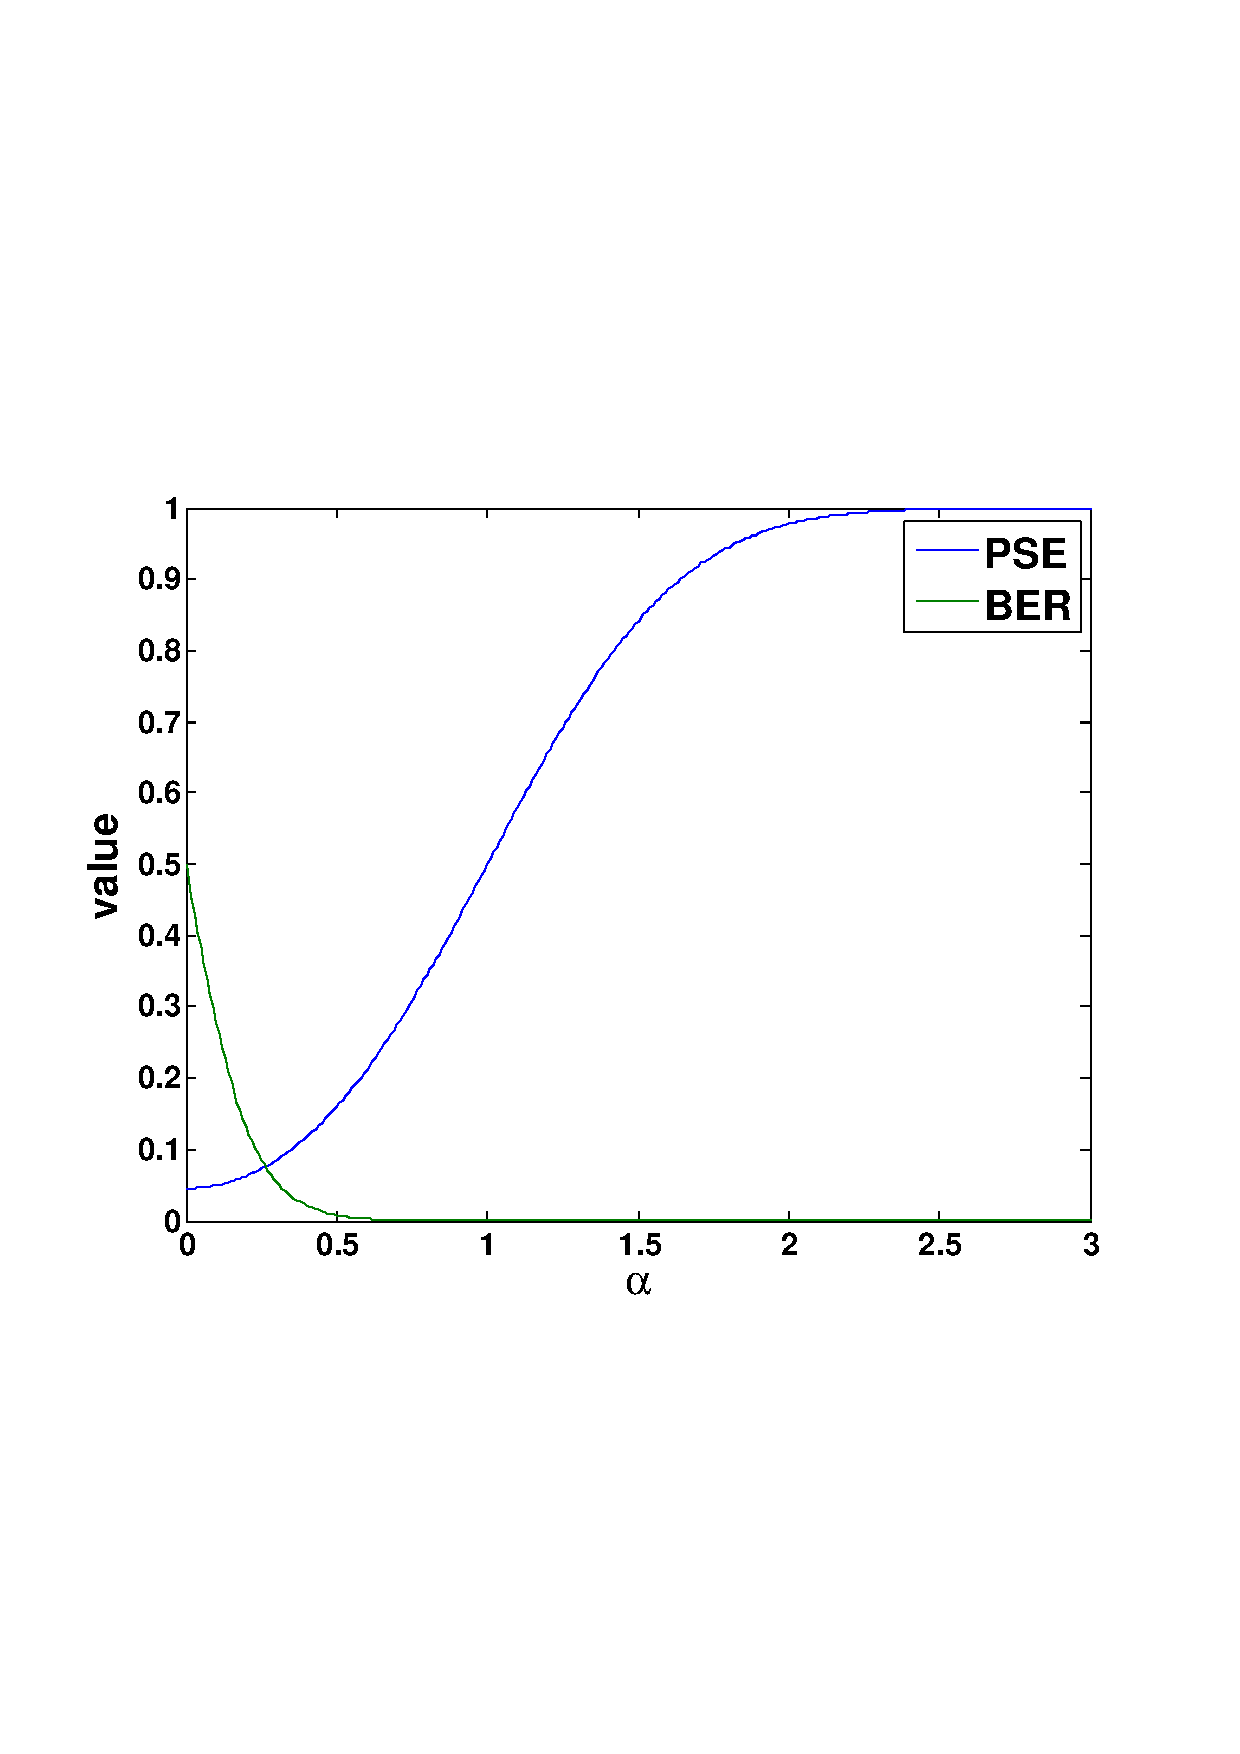
\includegraphics[width=\linewidth, trim= 0mm 60mm 0mm 70mm]{./sdf/cv_system/figures/singlehomodyne.pdf}
\caption{BER and PSE in function of $\alpha$ for the single homodyne setup. $X_0=1$ was used}
\label{fig:ber}
\end{figure}



\subsubsection*{Double Homodyne setup}

In our proposed double homodyne protocol both quadratures are measured simultaneously, as such the concept of correct and wrong basis measurements has no value. Our protocol also makes use of a locally generated Local Oscillator (LO), obtained from a different laser than the one used to generate the signal, thus we have to take into account the phase drift between both lasers. High intensity reference pulses are sent periodically to allow for an estimation of the phase drift. The double homodyne setup requires the signal to be divided into the two utilized detectors, so each measurement is made on a coherent state with half the amplitude of the incoming signal $\alpha\rightarrow\frac{\alpha}{\sqrt{2}}$
\par
For each incoming pulse we measure quadratures $X_\phi$ and $Y_\phi$. $\phi$ has contributions from both the encoded angle, $\theta$, and the phase difference between lasers, $\epsilon$, we assume $\phi=\theta+\epsilon$. On the reference pulses no phase is encoded, that is $\theta=0$, thus $\epsilon$ can be estimated. Assuming $\epsilon$ doesn't change between a reference pulse and the following signal pulse, the measured quadratures can be cast into the originally sent quadratures $X_\theta$ and $Y_\theta$ via:
\begin{equation}
\begin{aligned}
X_\theta&=X_\phi\cos\epsilon-Y_\phi\sin\epsilon\\
Y_\theta&=X_\phi\sin\epsilon+Y_\phi\sin\epsilon
\end{aligned}
\end{equation}
Assuming an announcement of the coding basis, the density operators~\eqref{eq:statedensity1} and~\eqref{eq:statedensity2} still apply. We can now define the probability density of obtaining results $X_\theta$ and $Y_\theta$, assuming a state in the $X_1$ base was sent, as:
\begin{align}
\braket{X_\theta|\hat{\rho}_1|X_\theta}&= \frac{\sqrt{\frac{2}{\pi}}}{4}\left(e^{-2\left(x_\theta-\frac{\alpha}{\sqrt{2}}\cos\theta\right)^2}+e^{-2\left(x_\theta+\frac{\alpha}{\sqrt{2}}\cos\theta\right)^2}\right),\\
\braket{Y_\theta|\hat{\rho_1}|Y_\theta}&= \frac{\sqrt{\frac{2}{\pi}}}{4}\left(e^{-2\left(y_\theta-\frac{\alpha}{\sqrt{2}}\sin\theta\right)^2}+e^{-2\left(y_\theta+\frac{\alpha}{\sqrt{2}}\sin\theta\right)^2}\right).
\end{align}
\par
Now each state needs to satisfy two limit values, $X_0$ and $Y_0$, to be accepted. Thus, the PSE is now defined as:
\begin{equation}
\begin{aligned}
P_{DH}(X_0,Y_0,\alpha)&=\int^{-X_0}_{-\infty}\braket{X_\theta|\hat{\rho}_1|X_\theta}dx_\theta\int^{-Y_0}_{-\infty}\braket{Y_\theta|\hat{\rho}_1|Y_\theta}dy_\theta+\\
&\int_{X_0}^{\infty}\braket{X_\theta|\hat{\rho}_1|X_\theta}dx_\theta\int_{Y_0}^{\infty}\braket{Y_\theta|\hat{\rho}_1|Y_\theta}dy_\theta\\
&=\frac{1}{4}\left\lbrace\text{erfc}\left[\sqrt{2}\left(X_0-\frac{\alpha}{\sqrt{2}}\cos\theta\right)\right]+\text{erfc}\left[\sqrt{2}\left(X_0+\frac{\alpha}{\sqrt{2}}\cos\theta\right)\right]\right\rbrace\\
&\left\lbrace\text{erfc}\left[\sqrt{2}\left(Y_0-\frac{\alpha}{\sqrt{2}}\sin\theta\right)\right]+\text{erfc}\left[\sqrt{2}\left(Y_0+\frac{\alpha}{\sqrt{2}}\sin\theta\right)\right]\right\rbrace,
\end{aligned}
\end{equation}
The DH subscript denotes Double Homodyne. In a somewhat similar manner, the BER is now defined as:
\begin{equation}\label{eq:adaptedBER}
\begin{aligned}
Q_{DH}(X_0,Y_0,\alpha)&=\frac{1}{P_{DH}}\left(\int^{-X_0}_{-\infty}\left|\braket{X_\theta|\frac{\alpha}{\sqrt{2}}}\right|^2dx_\theta\int^{-Y_0}_{-\infty}\left|\braket{Y_\theta|\frac{\alpha}{\sqrt{2}}}\right|^2dy_\theta+\right.\\
&\left.\int_{X_0}^{\infty}\left|\braket{X_\theta|-\frac{\alpha}{\sqrt{2}}}\right|^2dx_\theta\int_{Y_0}^{\infty}\left|\braket{Y_\theta|-\frac{\alpha}{\sqrt{2}}}\right|^2dy_\theta\right)\\
&=\frac{1}{2P_{DH}}\text{erfc}\left[\sqrt{2}\left(X_0+\frac{\alpha}{\sqrt{2}}\cos\theta\right)\right]\text{erfc}\left[\sqrt{2}\left(Y_0+\frac{\alpha}{\sqrt{2}}sin\theta\right)\right],
\end{aligned}
\end{equation}
note that, in this definition for BER, only values $\theta\in\left[0,\frac{\pi}{2}\right]$ make sense (the sent state was $\alpha$).

\begin{figure}[h]
\centering
\begin{subfigure}{.48\linewidth}
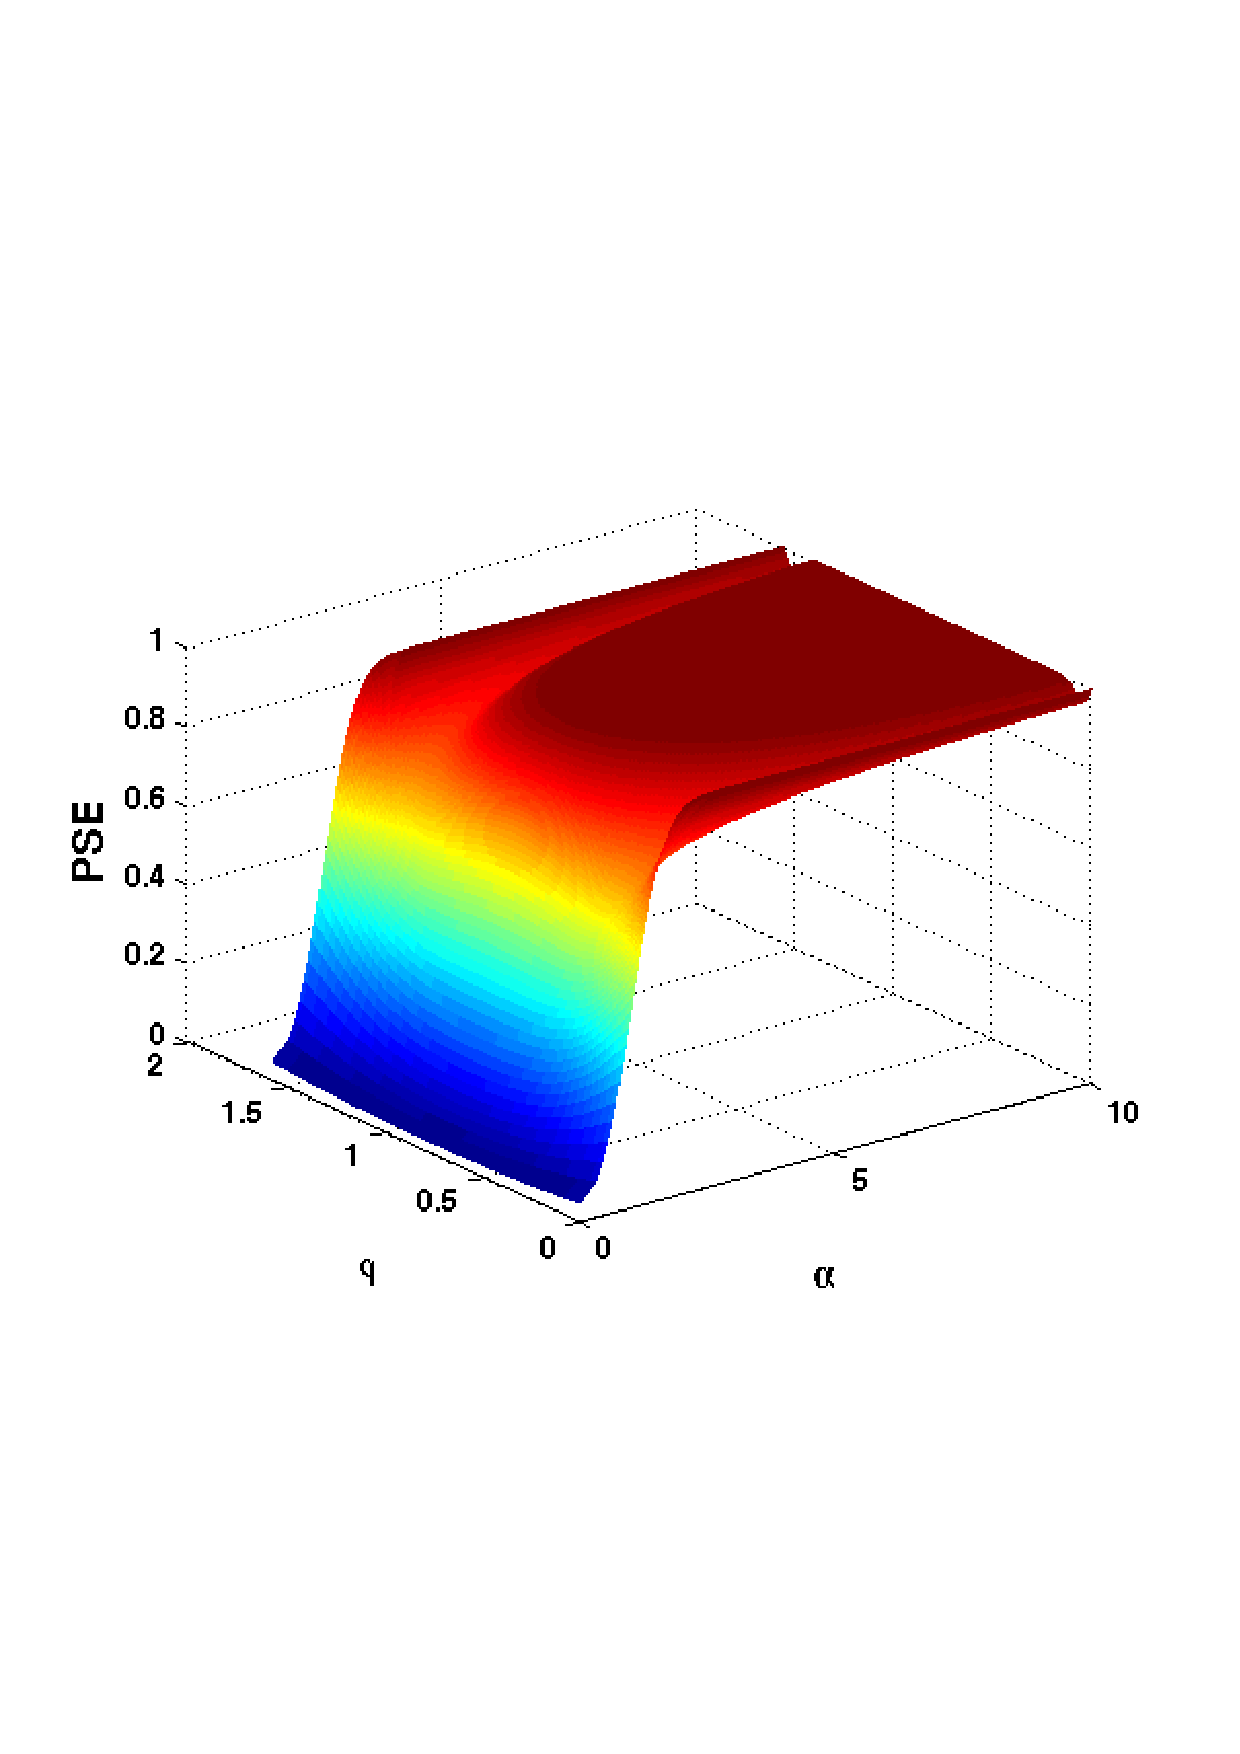
\includegraphics[width=\linewidth, trim= 0mm 60mm 0mm 70mm]{doublehomodynePSE.pdf}
\caption{PSE in function of $\alpha$ and $\theta$ for the double homodyne setup. $X_0=1$ was used}
\end{subfigure}
~
\begin{subfigure}{.48\linewidth}
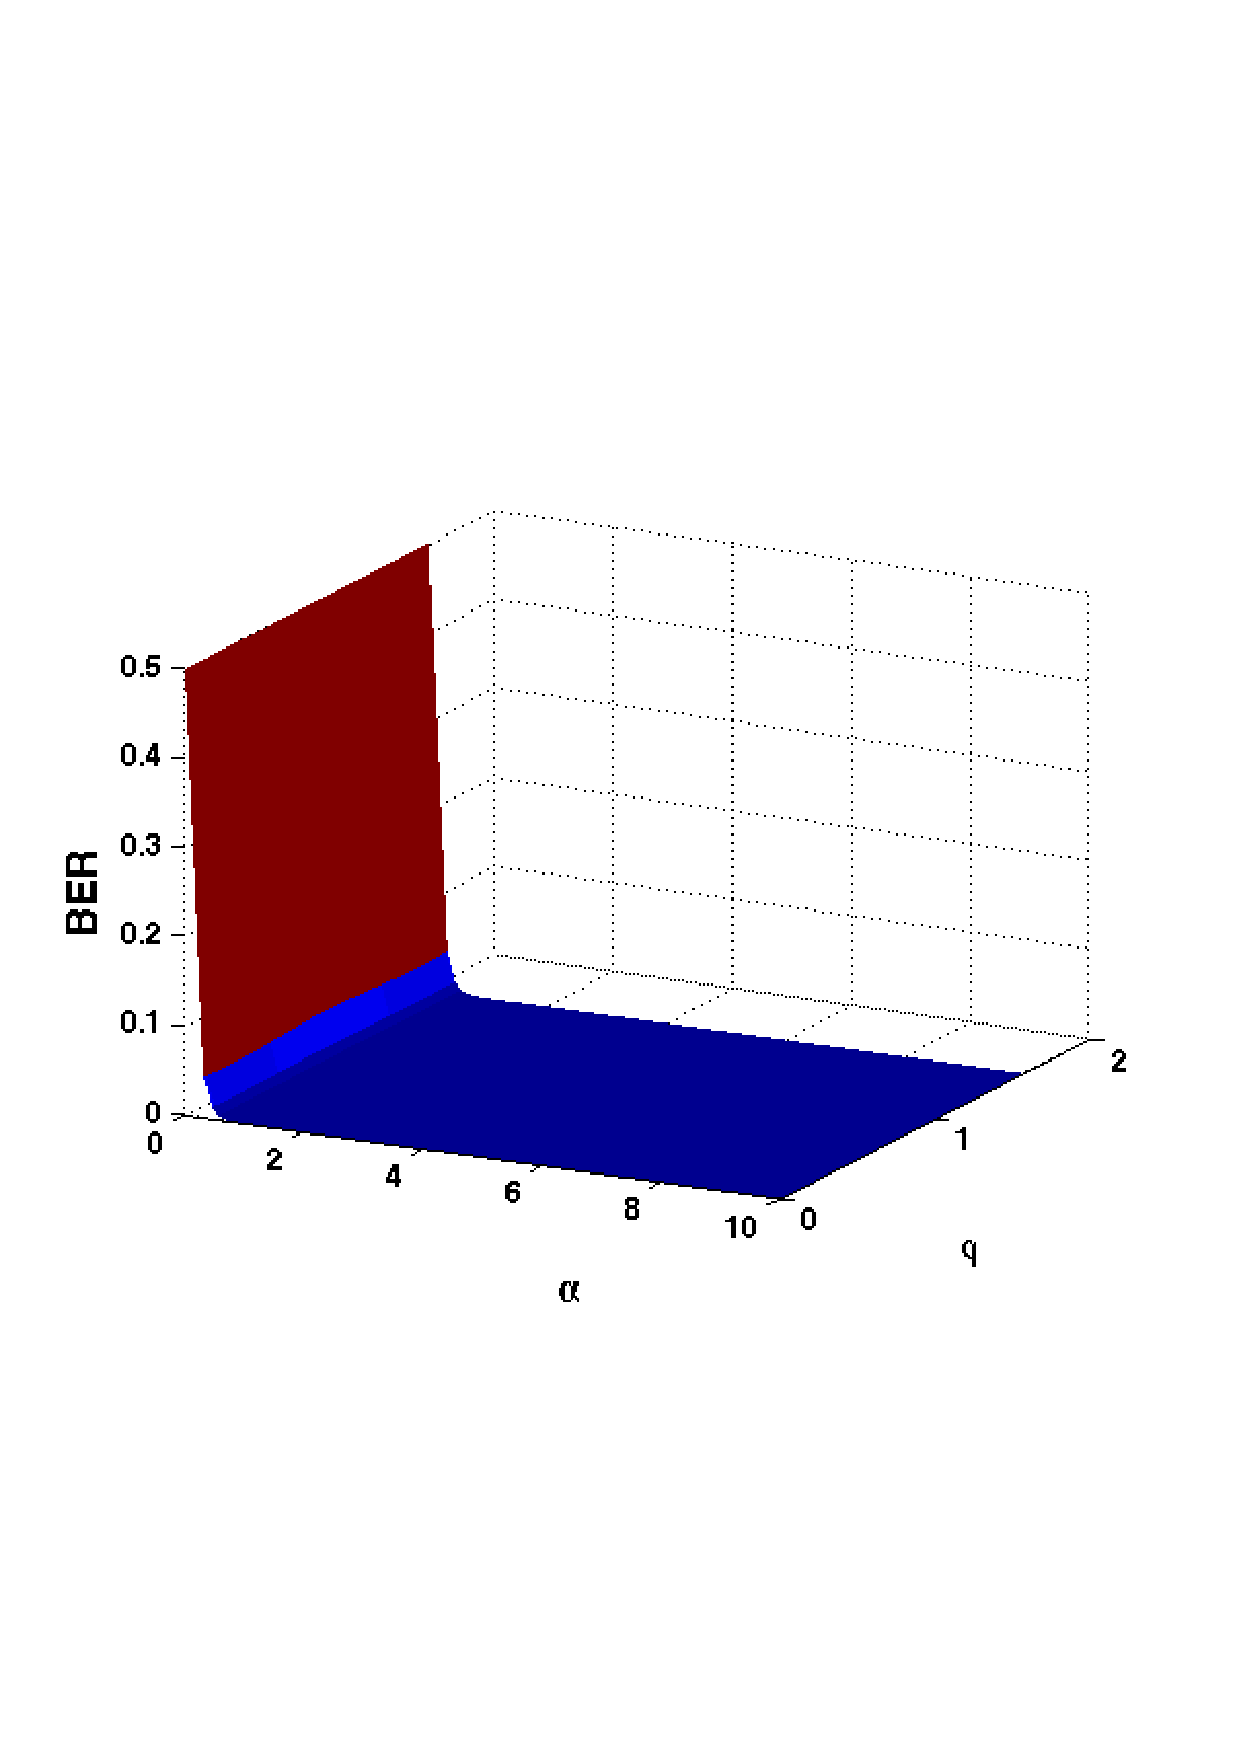
\includegraphics[width=\linewidth, trim= 0mm 60mm 0mm 70mm]{doublehomodyneBER.pdf}
\caption{BER in function of $\alpha$ and $\theta$ for the double homodyne setup. $X_0=1$ was used}
\end{subfigure}
\caption{Theoretical results for double homodyne setup.}
\end{figure}

\subsection*{Functional Description}

Simplified diagrams of the systems being simulated are presented in Figures~\ref{fig:singleH}. and~\ref{fig:doubleH}. Two optical signals are generated, one with a constant power level of 10~dBm and the other with power in multiples of the power corresponding to a single photon per sampling time (6.4078e$\times10^{-13}$~W for a sampling time of 200~ns). The two signals are mixed, with a Balanced Beam Splitter in the single homodyne case and with a 90$^\text{o}$ Optical Hybrid in the double homodyne one, and are subsequently evaluated with recourse to Homodyne Receivers.

\begin{figure}[h]
\centering
\begin{subfigure}{\linewidth}
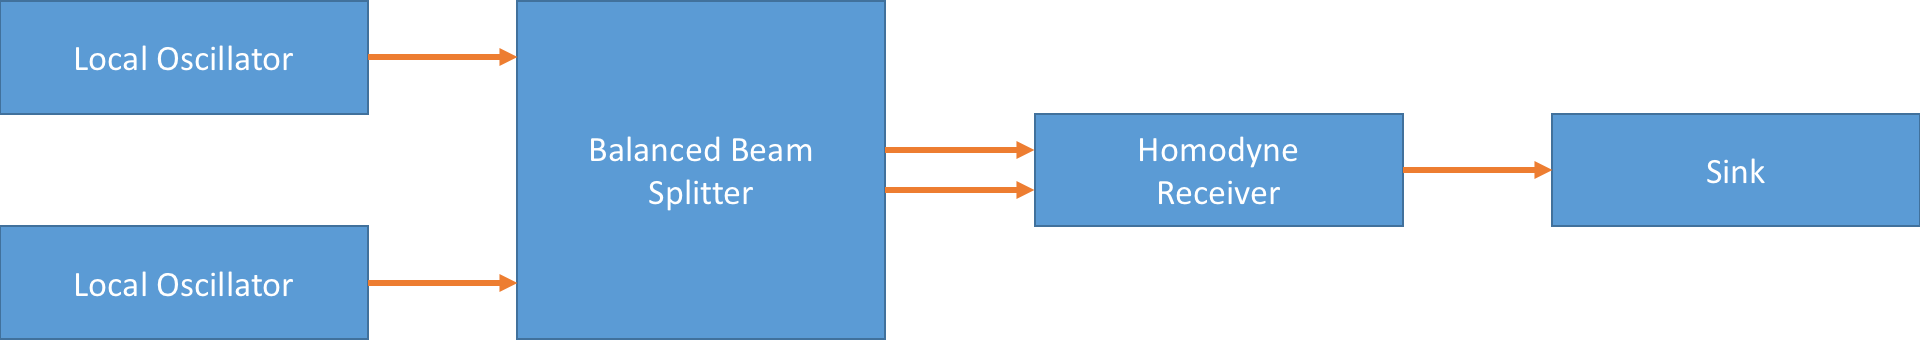
\includegraphics[width=\linewidth]{singlehomodyneSimuBlock.png}
\caption{Single homodyne simulation block diagram.}
\label{fig:singleH}
\end{subfigure}
\\
~
\\
\begin{subfigure}{\linewidth}
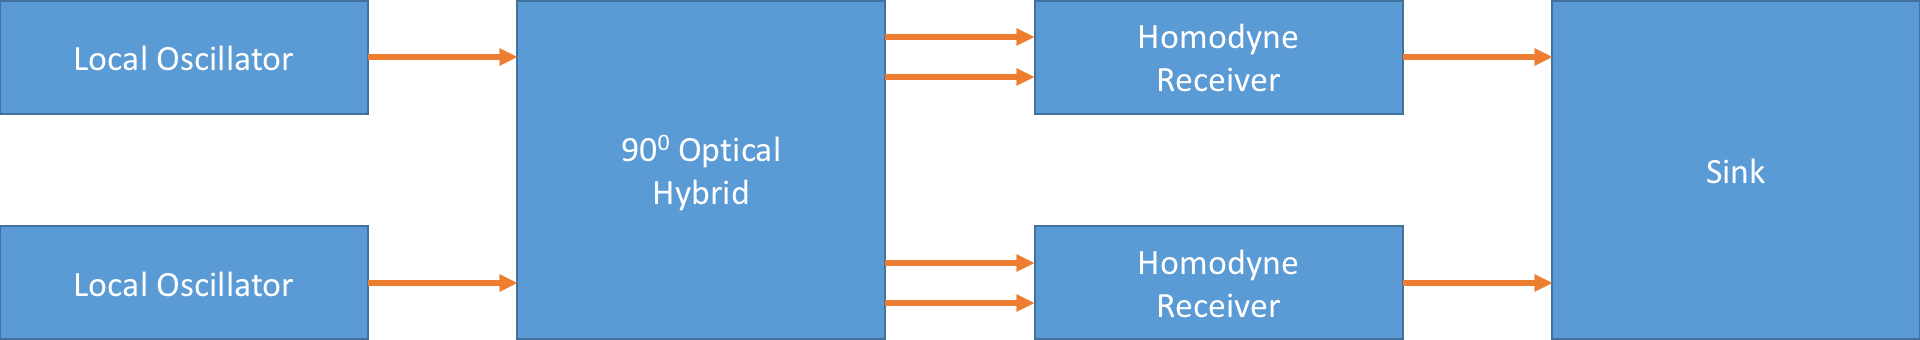
\includegraphics[width=\linewidth]{doublehomodyneSimuBlock.png}
\caption{Double homodyne simulation block diagram.}
\label{fig:doubleH}
\end{subfigure}
\caption{Block diagrams of both simulation results presented in this report.}
\end{figure}

\begin{table}[H]
\centering
\begin{tabular}{c|c}
System Blocks          & netxpto Blocks       \\ \hline
Local Oscillator       & LocalOscillator      \\
Homodyne Receiver      & I\_HomodyneReceiver   \\
Balanced Beam Splitter & BalancedBeamSplitter \\
90$^\text{o}$ Optical Hybrid     & OpticalHybrid
\end{tabular}
\end{table}

\pagebreak
\subsection*{Required files}\label{Required files}

Header Files
\begin{table}[H]
\centering
\begin{tabulary}{1.0\textwidth}{|L|L|}
\hline
\textbf{File}              & \textbf{Description} 				            \\ \hline
netxpto.h                  & Generic purpose simulator definitions.	        \\ \hline
local\_oscillator.h        & Generates continuous coherent signal.            \\ \hline
balanced\_beam\_splitter.h & Mixes the two input signals into two outputs.    \\ \hline
optical\_hybrid.h          & Mixes the two input signals into four outputs.   \\ \hline
homodyne\_reciever.h       & Performs coherent detection on the input signal. \\ \hline
sink.h                     & Closes any unused signals.                       \\ \hline
\end{tabulary}
\end{table}
%
Source Files
\begin{table}[H]
\centering
\begin{tabulary}{1.0\textwidth}{|L|L|}
\hline
\textbf{File}                & \textbf{Description} 					          \\ \hline
netxpto.cpp                  & Generic purpose simulator definitions.	          \\ \hline
local\_oscillator.cpp        & Generates continuous coherent signal.            \\ \hline
balanced\_beam\_splitter.cpp & Mixes the two input signals into two outputs.    \\ \hline
optical\_hybrid.cpp          & Mixes the two input signals into four outputs.   \\ \hline
homodyne\_reciever.cpp       & Performs coherent detection on the input signal. \\ \hline
sink.cpp                     & Closes any unused signals.                       \\ \hline
\end{tabulary}
\end{table}


\subsection*{System Input Parameters}

This system takes into account the following input parameters:
\begin{table}[H]
\centering
\begin{tabulary}{1.0\textwidth}{|C|C|}
\hline
\textbf{System Parameters} & \textbf{Description}                                                                   \\ \hline
numberOfBitsGenerated      & Gives the number of bits to be simulated                                               \\ \hline
bitPeriod                  & Sets the time between adjacent bits                                                    \\ \hline
samplesPerSymbol           & Establishes the number of samples each bit in the string is given                      \\ \hline
localOscillatorPower\_dBm1 & Sets the optical power, in units of dBm, at the reference output	                      \\ \hline
localOscillatorPower2      & Sets the optical power, in units of W, of the signal                                   \\ \hline
localOscillatorPhase1      & Sets the initial phase of the local oscillator used for reference                      \\ \hline
localOscillatorPhase2      & Sets the initial phase of the local oscillator used for signal                         \\ \hline
transferMatrix             & Sets the transfer matrix of the beam splitter used in the homodyne detector            \\ \hline
responsivity               & Sets the responsivity of the photodiodes used in the homodyne detector                 \\ \hline
amplification              & Sets the amplification of the trans-impedance amplifier used in the homodyne detector  \\ \hline
electricalNoiseAmplitude   & Sets the amplitude of the gaussian thermal noise added in the homodyne detector        \\ \hline
shotNoise                  & Chooses if quantum shot noise is used in the simulation                                \\ \hline
\end{tabulary}
\end{table}		

\subsection*{Inputs}

This system takes no inputs.
%
\subsection*{Outputs}

The single homodyne system outputs the following objects:
\begin{itemize}
\item Signals:
\begin{itemize}
\item Local Oscillator Optical Reference; (S$_{1}$)
\item Local Oscillator Optical Signal; (S$_{2}$)
\item Beam Splitter Outputs; (S$_{3}$, S$_{4}$)
\item Homodyne Detector Electrical Output; (S$_{5}$)
\end{itemize}
\end{itemize}
\par
The double homodyne system outputs the following objects:
\begin{itemize}
\item Signals:
\begin{itemize}
\item Local Oscillator Optical Reference; (S$_{1}$)
\item Local Oscillator Optical Signal; (S$_{2}$)
\item 90$^\text{o}$ Optical Hybrid Outputs; (S$_{3}$, S$_{4}$, S$_{5}$, S$_{6}$)
\item Homodyne Detector Electrical Output; (S$_{7}$)
\end{itemize}
\end{itemize}		

\subsection*{Simulation Results}
\subsubsection*{Single homodyne results}\label{subsec:SHresults}

The numerical results presented in Figure~\ref{fig:directber} were obtained with the simulation described by the block diagram in Figure~\ref{fig:singleH}. Theoretical results are a direct trace of~\eqref{eq:biterrorratio}. One can see that the numerical results adhere quite well to the expected curve.

\begin{figure}[h]
\centering
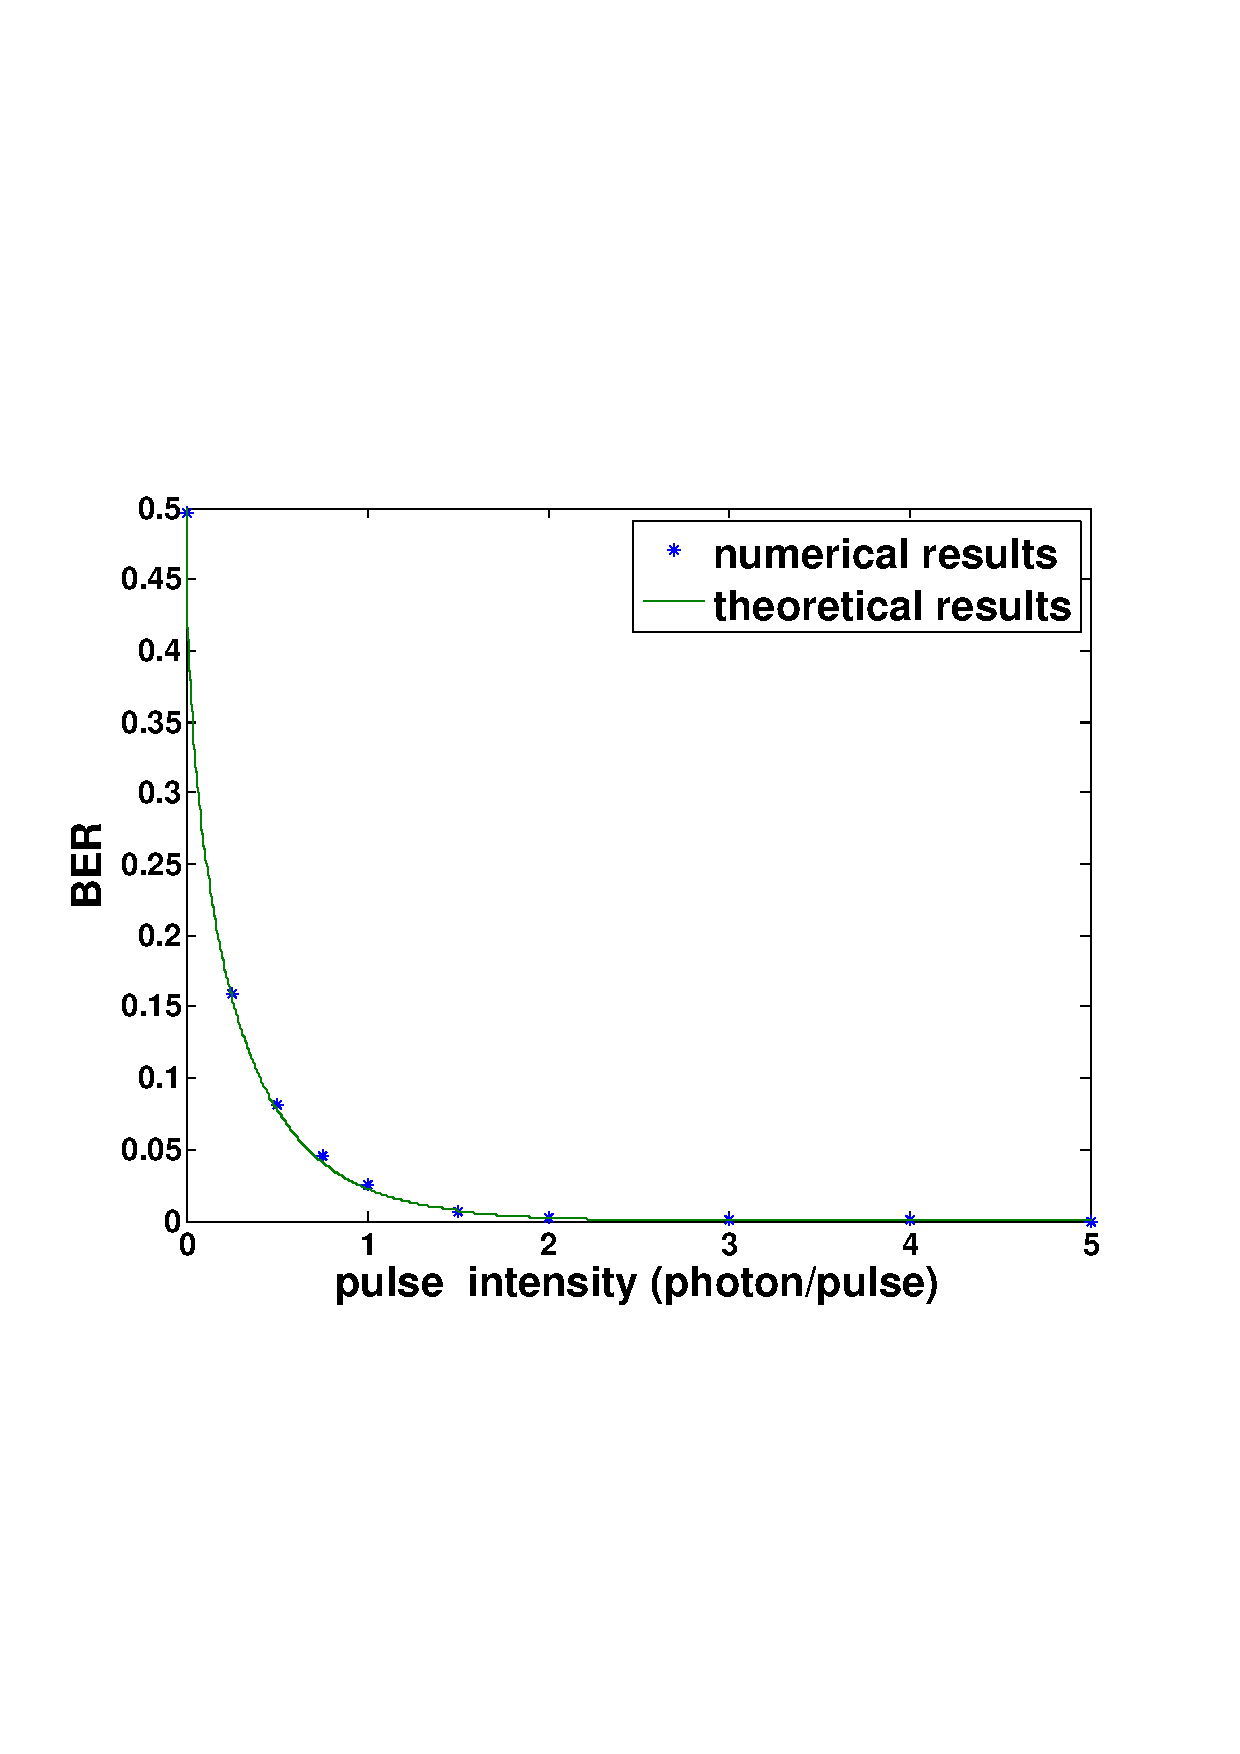
\includegraphics[width=\linewidth, trim= 0mm 60mm 0mm 70mm]{directBER.pdf}
\caption{BER in function of $\alpha$ for the single homodyne setup. $X_0=0$ was used}
\label{fig:directber}
\end{figure}

\subsubsection*{Double homodyne results}\label{subsec:DHresults}

The numerical results presented in Figure~\ref{fig:adaptedber} were obtained with the simulation described by the block diagram in Figure~\ref{fig:doubleH}. Theoretical results are a direct trace of~\eqref{eq:adaptedBER} with $\theta=\frac{\pi}{4}$. One can see that the numerical results adhere quite well to the expected curve.

\begin{figure}[h]
\centering
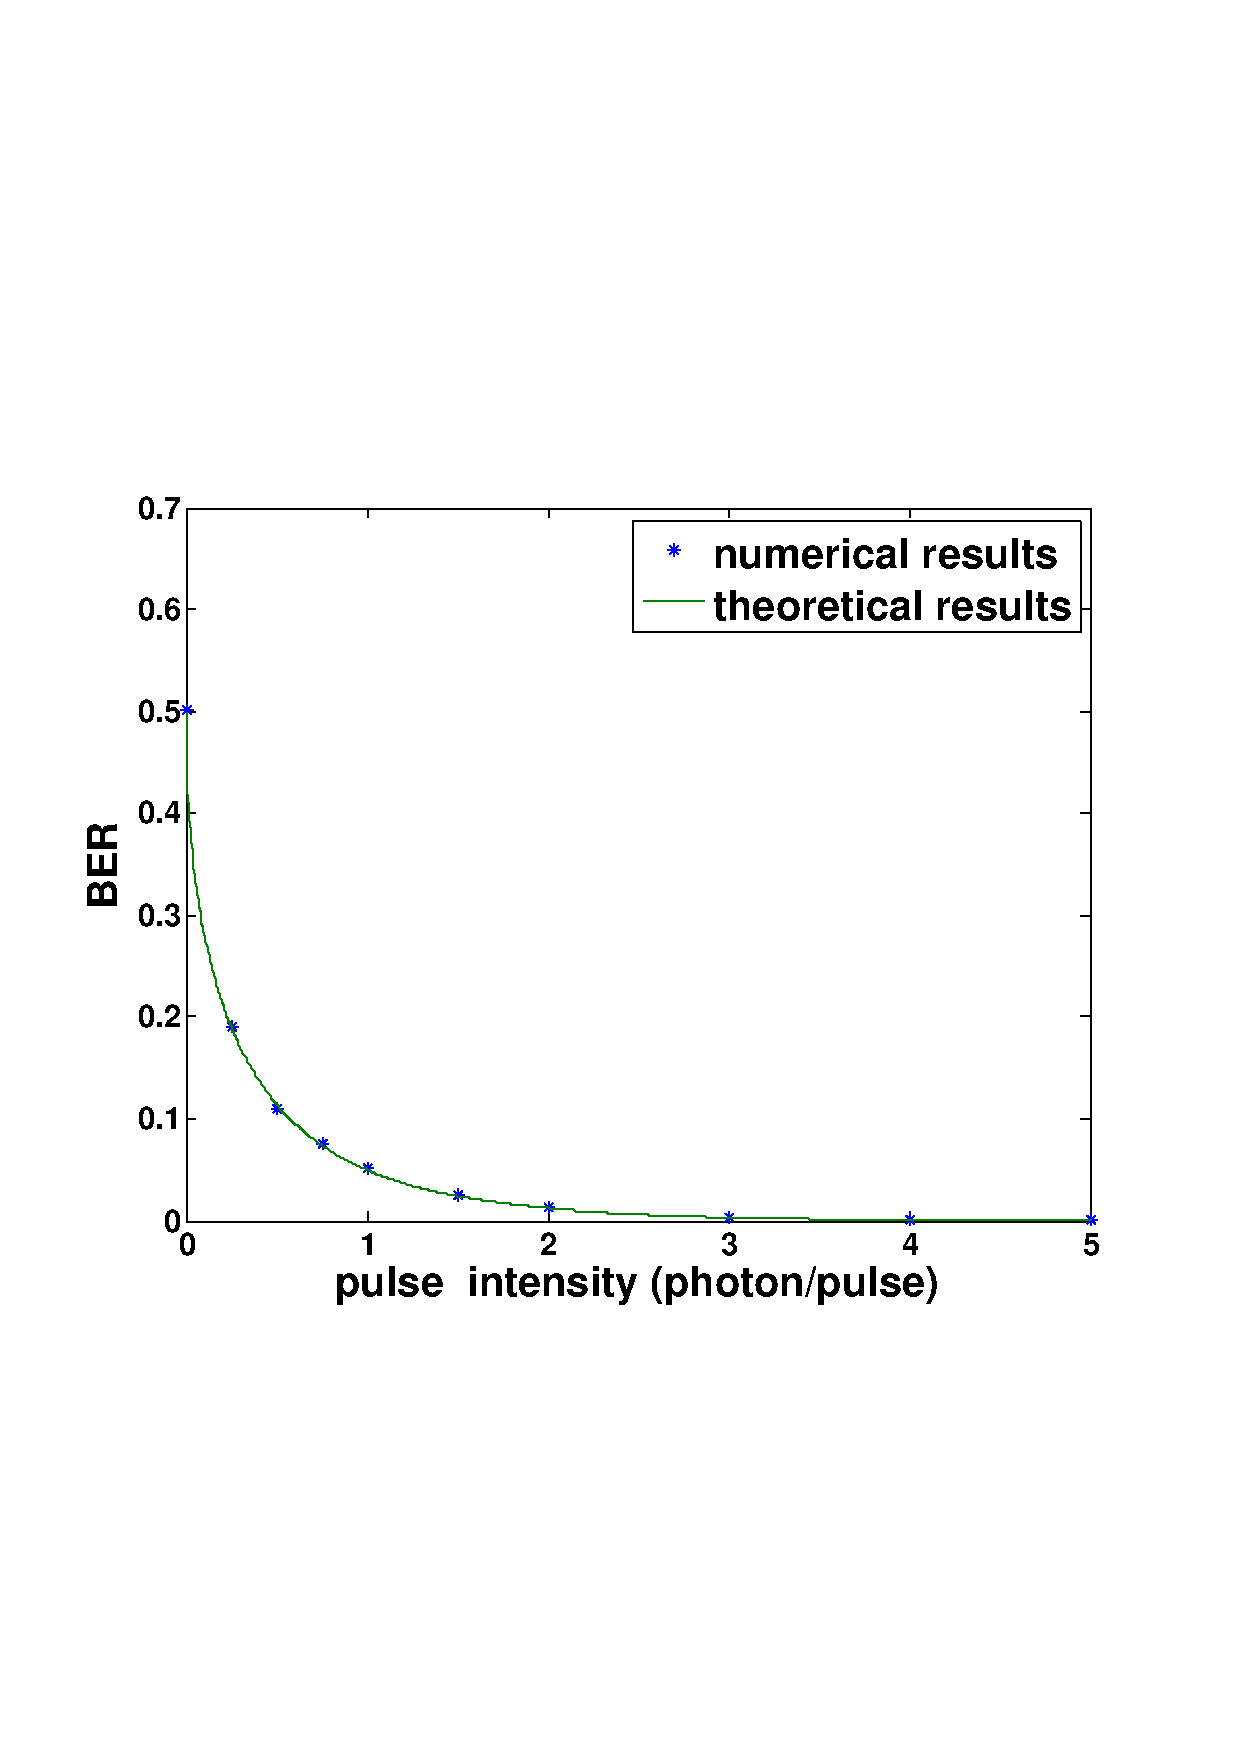
\includegraphics[width=\linewidth, trim= 0mm 60mm 0mm 70mm]{adaptedBER.pdf}
\caption{BER in function of $\alpha$ for the double homodyne setup. $X_0=0$ was used}
\label{fig:adaptedber}
\end{figure}

%\section{Block Description}
%
%\subsection{Homodyne Receiver}
%\subfile{./lib/i_homodyne_receiver}
%
%\subsection{Local Oscillator}
%\subfile{./lib/localoscillator}
%
%\subsection{Beam Splitter}
%\subfile{./lib/beamsplitter}
%
%\subsection{90$^\text{o}$ Optical Hybrid}
%
%\subsection{Photodiode}
%\subfile{./lib/photodiode}
%
%\subsection{Amplifier}
%\subfile{./lib/ideal_amplifier}
%
%\subsection{Electrical Filter}
%\subfile{./lib/pulse_shaper}

\subsection*{Known Problems}
\begin{enumerate}
    \item Homodyne Super-Block not functioning
    \item 90$^\text{o}$ Optical Hybrid PDF needs to be written
\end{enumerate}


\bibliographystyle{unsrt}
\bibliography{bibliography}
%\end{document} 
%\include{../sdf/TexFiles/EnquadramentoVHDL}
%\include{CapacidadeTeoriacadeTransmitirInformacao}
%\include{SistemasCoerentesComDSP}
%\include{SistemasMultiMode}
%\include{SistemasComunicacaoQuanticos}
%\include{Conclusao}
%\appendix
%\include{Acronymous}
%\printindex

%   create the appendix and include it


\pagebreak

%--------------------------------- SECTION ----------------------------------
\bibliographystyle{ieeetr}
% argument is your BibTeX string definitions and bibliography database(s)
%\bibliography{../../../Computadores/Bibtex/IEEEabrv,../../../Computadores/Bibtex/AnpBib}


\printglossaries

\end{document}
